%%%%%%%%%%%%%%%%%%%%%%%%%%%%%%%%%%%%%%%%%%%%%%%%%%%%%%%%%%%%%%%%%%%%%%
% Overleaf (WriteLaTeX) Example: Molecular Chemistry Presentation
%
% Source: http://www.overleaf.com
%
% In these slides we show how Overleaf can be used with standard 
% chemistry packages to easily create professional presentations.
% 
% Feel free to distribute this example, but please keep the referral
% to overleaf.com
% 
%%%%%%%%%%%%%%%%%%%%%%%%%%%%%%%%%%%%%%%%%%%%%%%%%%%%%%%%%%%%%%%%%%%%%%

\documentclass{beamer}

\mode<presentation>
{
  \usetheme{Madrid}       % or try default, Darmstadt, Warsaw, ...
  \usecolortheme{default} % or try albatross, beaver, crane, ...
  \usefonttheme{default}    % or try default, structurebold, ...
  \setbeamertemplate{navigation symbols}{}
  \setbeamertemplate{caption}[numbered]
} 

\usepackage[english]{babel}
\usepackage[utf8x]{inputenc}
\usepackage{graphicx}
\usepackage{hyperref}
  \hypersetup{colorlinks=true}
  \hypersetup{urlcolor=blue}
  \hypersetup{linkcolor = .}
\usepackage{xcolor}
\usepackage{siunitx}
  \sisetup{separate-uncertainty = true}
\usepackage{physics}
\usepackage[font=small,labelfont=bf]{caption}
\usepackage{subcaption}
\usepackage[en-GB]{datetime2}
\usepackage{overpic}
\usepackage{feynmp}
\DeclareGraphicsRule{*}{mps}{*}{}
\usepackage{scalerel}
\newcommand{\mylbrace}[2]{\vspace{#2pt}\hspace{6pt}\scaleleftright[\dimexpr5pt+#1\dimexpr0.06pt]{\lbrace}{\rule[\dimexpr2pt-#1\dimexpr0.5pt]{-4pt}{#1pt}}{.}}
\newcommand{\myrbrace}[2]{\vspace{#2pt}\scaleleftright[\dimexpr5pt+#1\dimexpr0.06pt]{.}{\rule[\dimexpr2pt-#1\dimexpr0.5pt]{-4pt}{#1pt}}{\rbrace}\hspace{6pt}}

% Here's where the presentation starts, with the info for the title slide
\title[$B^\pm\to(K^+K^-\pi^+\pi^-)_Dh^\pm$]{A study of CP violation in \texorpdfstring{$B^\pm\to(K^+K^-\pi^+\pi^-)_Dh^\pm$}{B to K+K-pi+pi-} and \texorpdfstring{$B^\pm\to(\pi^+\pi^-\pi^+\pi^-)_Dh^\pm$}{B to K+K-pi+pi-} decays}

\author{\textbf{Martin Tat} \hspace{0.54em} Guy Wilkinson \hspace{0.54em} Sneha Malde}
\institute{\normalsize University of Oxford \\ \vspace{0.3cm} \normalsize Approval presentation \vspace{-0.2cm}}
\date{2nd September 2022}

\titlegraphic{
\includegraphics[height = 2cm]{lhcb.jpg}\hspace{2cm}~%
              
\includegraphics[height = 2cm]{OxfordLogo.pdf}}

\begin{document}

\begin{frame}
  \titlepage
\end{frame}

% These three lines create an automatically generated table of contents.
%\begin{frame}{Outline}
%  \tableofcontents
%\end{frame}

\section{Thank you}

\begin{frame}{Thank you}
  \begin{itemize}
    \setlength\itemsep{2.0em}
    \item{Big thank you to all reviewers!}
    \item{B2OC WG reviewers/convenors:}
    \begin{itemize}
      \item{Anton Poluektov}
      \item{Nathan Philip Jurik}
      \item{Paras Naik}
    \end{itemize}
    \item{RC reviewers:}
    \begin{itemize}
      \item{Lucia Grillo}
      \item{Francesco Dettori}
    \end{itemize}
  \end{itemize}
\end{frame}

\section{Introduction and motivation}

\begin{frame}{Introduction and motivation}
  \begin{itemize}
    \setlength\itemsep{0.0em}
    \item{Aim of this analysis: Measure CP observables in $B^\pm\to[K^+K^-\pi^+\pi^-]_D h^\pm$, $h = K, \pi$ decays}
    \begin{itemize}
      \setlength\itemsep{0.5em}
      \item{First study of CP violation in this channel}
      \item{Enhance sensitivity through sophisticated binning of 5D phase space}
      \item{Provide input for future model-independent measurement of $\gamma$}
    \end{itemize}
    \item{Also measure phase space inclusive CP observables for $B^\pm\to[\pi^+\pi^-\pi^+\pi^-]_D h^\pm$, $h = K, \pi$ decays}
  \end{itemize}
  \vspace{-0.2cm}
  \begin{figure}
    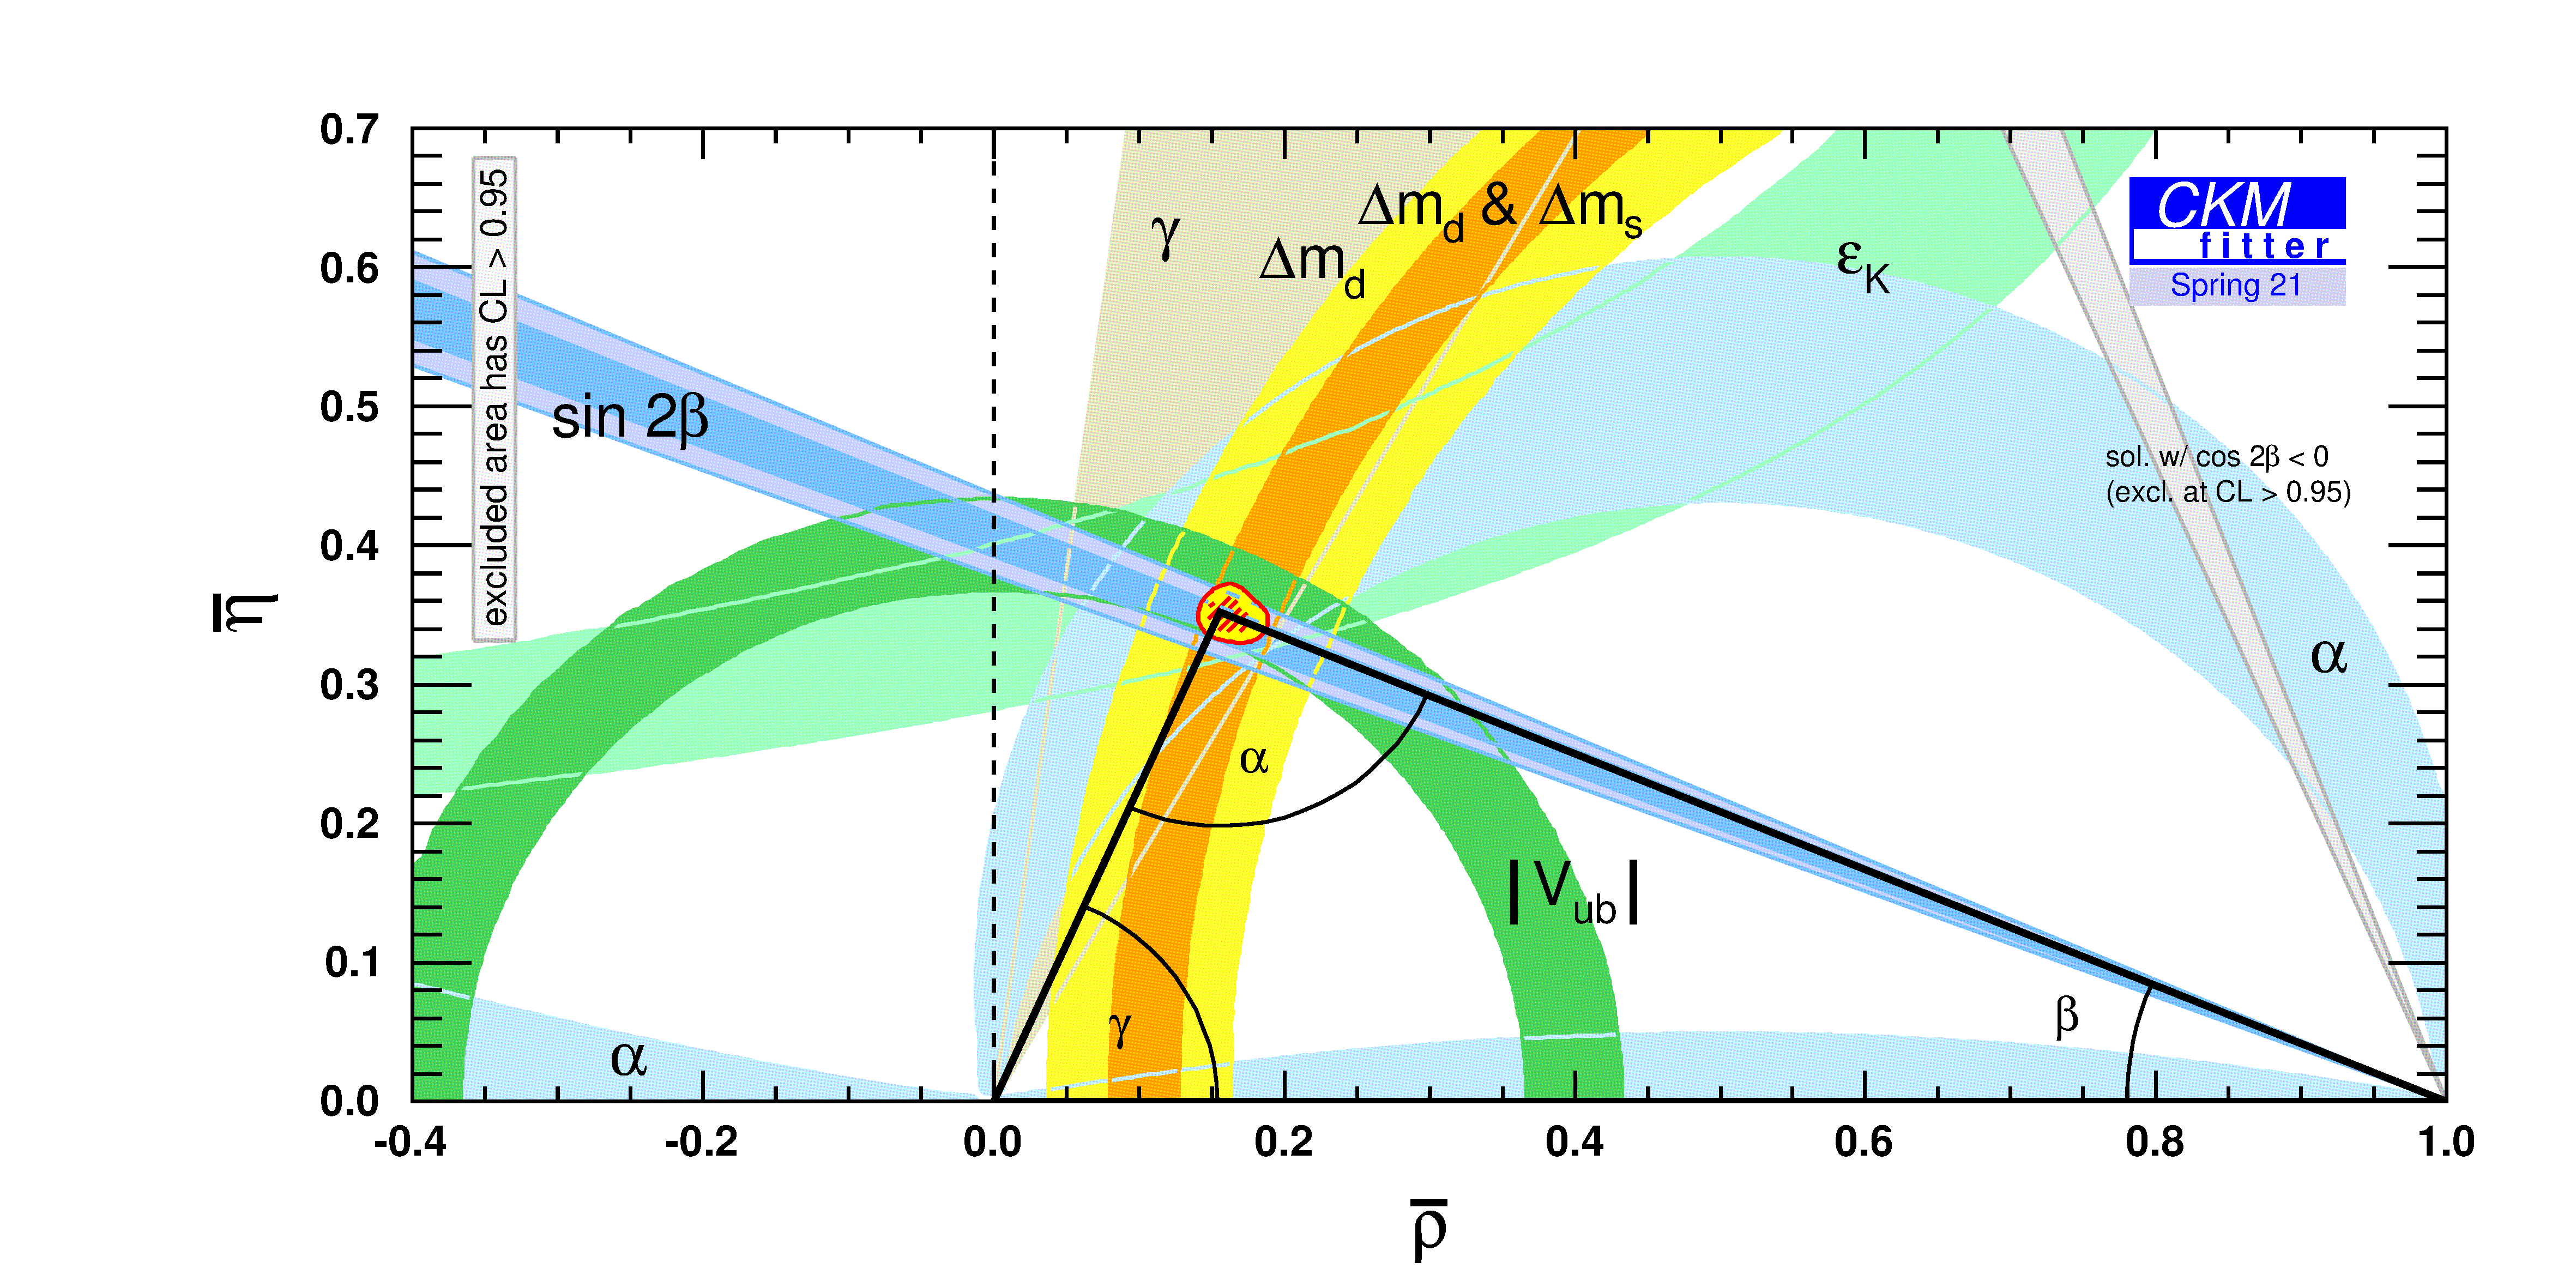
\includegraphics[width = 0.70\textwidth]{Plots/ckmfitter2.png}
  \end{figure}
  \vspace{-0.5cm}
  \begin{center}
    \tiny{CKMfitter Group (J. Charles et al.), Eur. Phys. J. C41, 1-131 (2005)}
  \end{center}
\end{frame}

\begin{frame}{Introduction and motivation}
  \vspace{0.5cm}
  \begin{itemize}
    \setlength\itemsep{1.5em}
    \item{$B^\pm\to[K^+K^-\pi^+\pi^-]_D K^\pm$ was first proposed by J. Rademacker and G. Wilkinson}
    \begin{itemize}
      \item{\href{https://arxiv.org/abs/hep-ph/0611272}{Phys. Lett. B647 (2007) 400}}
      \item{Expected $\gamma$ precision from FOCUS amplitude model with $1000$ $B^\pm\to DK^\pm$ candidates: $14^\circ$}
    \end{itemize}
    \item{Recent state of the art amplitude analysis by LHCb:}
    \begin{itemize}
      \item{\href{https://arxiv.org/abs/1811.08304}{JHEP 02 (2019) 126}}
      \item{Develop a suitable binning scheme}
    \end{itemize}
    \item{No measurement of strong phases $c_i$ and $s_i$ exists today}
    \begin{itemize}
      \item{Current BESIII dataset is $8$~fb$^{-1}$}
      \item{Allows for a direct measurement of $D\to K^+K^-\pi^+\pi^-$ strong phases}
      \item{Final $\gamma$ measurement will be model independent}
    \end{itemize}
  \end{itemize}
\end{frame}

\section{Theory of BPGGSZ method}

\begin{frame}{Theory of BPGGSZ method}
  \begin{itemize}
    \item{$B^\pm\to Dh^\pm$ amplitude:}
  \end{itemize}
  \begin{center}
    $\mathcal{A}(B^-) = \mathcal{A}(D^0) + r_Be^{i(\delta_B - \gamma)}\mathcal{A}(\bar{D^0})$ \\
    $\mathcal{A}(B^+) = \mathcal{A}(\bar{D^0}) + r_Be^{i(\delta_B + \gamma)}\mathcal{A}(D^0)$ \\
  \end{center}
  \begin{itemize}
    \item{$\mathcal{A}(D^0)$ and $\mathcal{A}(\bar{D^0})$ depend on $D$ phase space}
    \item{Strong-phase difference of $D^0$ and $\bar{D^0}$ decays inaccessible at LHCb}
    \item{Model-independent measurement: Integrate over bins of phase space}
  \end{itemize}
  \begin{block}{Event yield in bin $i$}
    $N^-_i = h_{B^-}\Big(F_i + \big(x_-^2 + y_-^2\big)\bar{F_i} + 2\sqrt{F_i\bar{F_i}}\big(x_-c_i + y_-s_i\big)\Big)$
    $N^+_{-i} = h_{B^+}\Big(F_i + \big(x_+^2 + y_+^2\big)\bar{F_i} + 2\sqrt{F_i\bar{F_i}}\big(x_+c_i + y_+s_i\big)\Big)$
  \end{block}
\end{frame}

\begin{frame}{Theory of BPGGSZ method}
  \begin{block}{Event yield in bin $i$}
    \scriptsize
    $N^-_i = h_{B^-}\big(F_i + (x_-^2 + y_-^2)\bar{F_i} + 2\sqrt{F_i\bar{F_i}}(x_-c_i + y_-s_i)\big)$ \\
    $N^+_{-i} = h_{B^+}\big(F_i + (x_+^2 + y_+^2)\bar{F_i} + 2\sqrt{F_i\bar{F_i}}(x_+c_i + y_+s_i)\big)$
  \end{block}
  \begin{itemize}
    \item{CP observables:}
    \begin{itemize}
      \item{$x_\pm^{DK} = r_B^{DK}\cos(\delta_B^{DK}\pm\gamma)$, \quad $y_\pm^{DK} = r_B^{DK}\sin(\delta_B^{DK}\pm\gamma)$}
      \item{$x_\xi^{D\pi} = \Re(\xi^{D\pi})$, $y_\xi^{D\pi} = \Im(\xi^{D\pi})$ $\quad\quad\Big(\xi^{D\pi} = \frac{r_B^{D\pi}}{r_B^{DK}}e^{i(\delta_B^{D\pi} - \delta_B^{DK})}\Big)$}
    \end{itemize}
    \item{Fractional bin yield:}
    \begin{itemize}
      \item{$F_i = \frac{\int_i\dd{\Phi}|\mathcal{A}(D^0)|^2}{\sum_j\int_j\dd{\Phi}\abs{\mathcal{A}(D^0)}^2}$}
      \item{Floated in the fit, mostly constrained by $B^\pm\to D\pi^\pm$}
    \end{itemize}
  \end{itemize}
  \begin{itemize}
    \item{Amplitude averaged strong phases:}
    \begin{center}
      $c_i = \frac{\int_i\dd{\Phi}|\mathcal{A}(D^0)||\mathcal{A}(\bar{D^0})|\cos(\delta_D)}{\sqrt{\int_i\dd{\Phi}\abs{\mathcal{A}(D^0)}^2\int_i\dd{\Phi}\abs{\mathcal{A}(\bar{D^0})}^2}}$ \quad $s_i = \frac{\int_i\dd{\Phi}|\mathcal{A}(D^0)||\mathcal{A}(\bar{D^0})|\sin(\delta_D)}{\sqrt{\int_i\dd{\Phi}\abs{\mathcal{A}(D^0)}^2\int_i\dd{\Phi}\abs{\mathcal{A}(\bar{D^0})}^2}}$
    \end{center}
  \end{itemize}
\end{frame}

\section{Binning scheme}

\begin{frame}{Binning scheme}
  \vspace{0.0cm}
  {\Large A binning scheme must satisfy the following:}
  \begin{itemize}
    \item{Minimal dilution of strong phases when integrating over bins}
    \item{Enhance interference between $B^\pm\to D^0h^\pm$ and $B^\pm\to\bar{D^0}h^\pm$}
  \end{itemize}
  \vspace{0.4cm}
  {\Large How to bin a 5-dimensional phase space?}
  \begin{itemize}
    \item{Generate C++ code for LHCb amplitude model using AmpGen\footnote{\href{https://github.com/GooFit/AmpGen}{AmpGen} by Tim Evans}}
    \item{For each $B^\pm$ candidate, calculate}
  \end{itemize}
  \begin{center}
    {\Large $\frac{\mathcal{A}(D^0)}{\mathcal{A}(\bar{D^0})} = r_De^{i\delta_D}$}
  \end{center}
  \begin{itemize}
    \item{Bin along $\delta_D$ and $r_D$, maximize $Q$-value to optimize}
    \begin{itemize}
      \item{$Q = 1$ corresponds to unbinned limit}
    \end{itemize}
  \end{itemize}
\end{frame}

\begin{frame}{Binning scheme}
  \begin{figure}
    \centering
    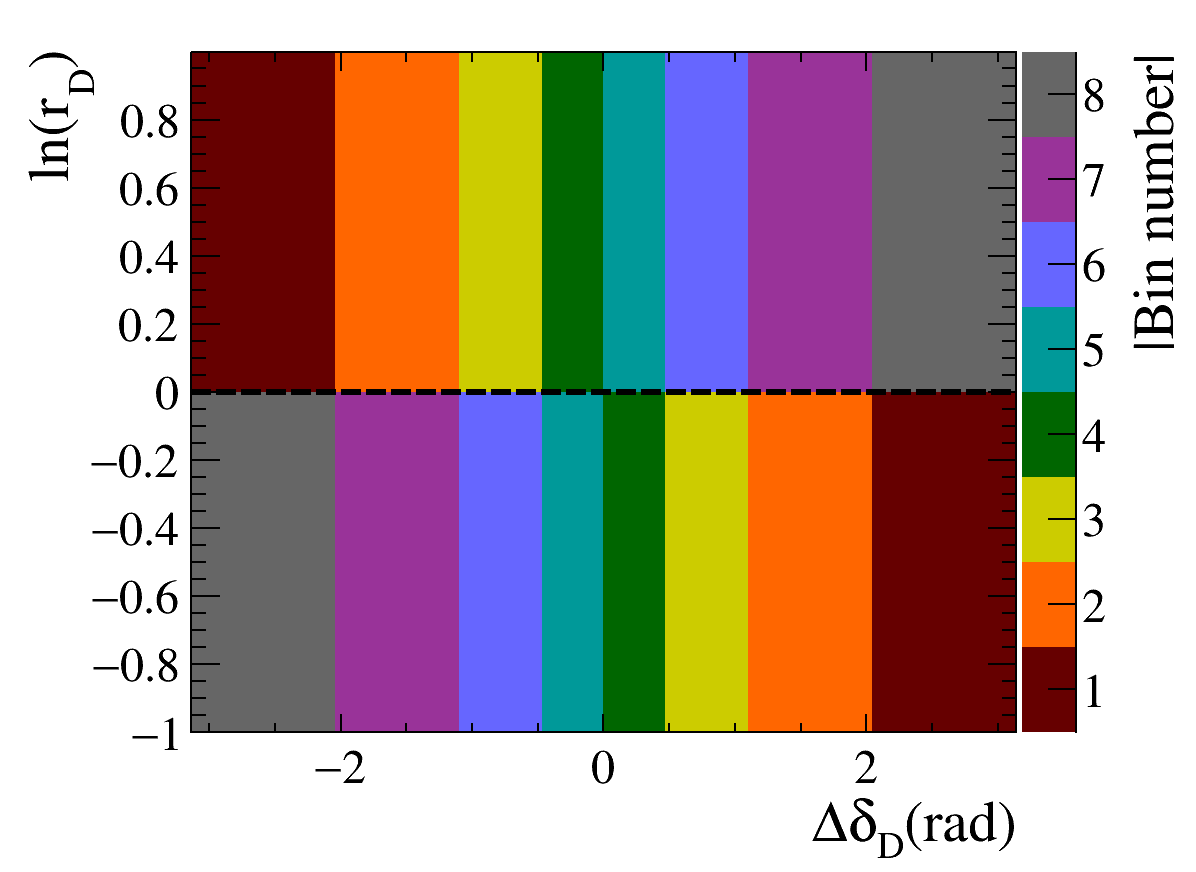
\includegraphics[width = 0.7\textwidth]{Plots/BinningSchemePlot_8Bins.png}
  \end{figure}
  \vspace{-1.0cm}
  \begin{center}
    $Q = 0.90$ \\
    Bins $i < 0$ on top, $i > 0$ below
  \end{center}
\end{frame}

\section{Quasi-GLW method}

\begin{frame}{Phase-space inclusive CP observables}
  \begin{itemize}
    \setlength\itemsep{0.5em}
    \item{Statistically independent analysis without phase space binning}
    \begin{itemize}
      \item{BPGGSZ looks at relative bin yields}
      \item{Quasi-GLW observables depend on absolute yields}
    \end{itemize}
    \item{Charge asymmetry:}
    \begin{center}
      $A_h = \frac{\Gamma(B^-\to D h^-) - \Gamma(B^+\to D h^+)}{\Gamma(B^-\to D h^-) + \Gamma(B^+\to D h^+)}$
    \end{center}
    \item{$B\to DK$ vs $B\to D\pi$ double ratio:}
    \begin{center}
      $R_{\rm CP} = \frac{R_{hh\pi\pi}}{R_{K\pi\pi\pi}}, \quad R = \frac{\Gamma(B^-\to D K^-) + \Gamma(B^+\to D K^+)}{\Gamma(B^-\to D\pi^-) + \Gamma(B^+\to D\pi^+)}$
    \end{center}
    \item{Measure $A_h$ and $R_{\rm CP}$ for $B^\pm\to[K^+K^-\pi^+\pi^-]_Dh^\pm$ and $B^\pm\to[\pi^+\pi^-\pi^+\pi^-]_Dh^\pm$}
  \end{itemize}
\end{frame}

\begin{frame}{Phase-space inclusive CP observables}
  \begin{block}{CP observables and physics parameters}
    $A_h = \frac{2r_B^{Dh}(2F_+ - 1)\sin(\delta_B^{Dh})\sin(\gamma)}{1 + (r_B^{Dh})^2 + 2r_B^{Dh}(2F_+ - 1)\cos(\delta_B^{Dh})\cos(\gamma)}$, \\~\\
    $R_{\rm CP} = 1 + (r_B^{Dh})^2 + 2r_B^{Dh}(2F_+ - 1)\cos(\delta_B^{Dh})\cos(\gamma)$
  \end{block}
  \vspace{0.3cm}
  \begin{itemize}
    \setlength\itemsep{0.5em}
    \item{Need CP-even fraction $F_+$ to interpret in terms of physics parameters}
    \item{For $D^0\to K^+K^-\pi^+\pi^-$:}
    \begin{itemize}
      \item{$F_+ = 0.736$}
      \item{Calculated from the model}
    \end{itemize}
    \item{For $D^0\to\pi^+\pi^-\pi^+\pi^-$:}
    \begin{itemize}
      \item{$F_+ = 0.735 \pm 0.016$}
      \item{Recent measurement by BESIII \href{https://arxiv.org/abs/2208.10098}{arXiv:2208.10098}}
    \end{itemize}
  \end{itemize}
\end{frame}

\section{Publication strategy}

\begin{frame}{Publication strategy}
  \begin{itemize}
    \setlength\itemsep{2.0em}
    \item{Strong phases $c_i$ and $s_i$ have not been published by BESIII yet}
    \item{We would like to publish a model dependent result initially}
    \begin{itemize}
      \item{Focus of the paper should be on CP violation, not $\gamma$}
      \item{Bin yields and correlation matrices will be provided in the appendix}
    \end{itemize}
    \item{When $c_i$ and $s_i$ become available, the result can be updated to yield a model independent measurement of $\gamma$, which can be included in the next combination}
  \end{itemize}
\end{frame}

\section{Selection}

\begin{frame}{Selection}
  \begin{enumerate}
    \setlength\itemsep{0.0em}
    \item{Initial cuts: Trigger requirements, mass cuts, bachelor $p$, etc}
    \begin{itemize}
      \item{$D$ mass window: $25$ MeV}
      \item{$B^\pm$ mass fit range: $[5080, 5700]$ MeV}
    \end{itemize}
    \item{BDT: Efficient combinatorial background rejection}
    \begin{itemize}
      \item{Signal sample: MC with AmpGen model}
      \item{Background sample: Data from $m_B\in[5800, 7000]$~MeV}
      \item{Pick BDT cut that minimises statistical sensitity of $\gamma$}
    \end{itemize}
    \item{Final cuts: PID cuts, flight significance cuts, $K_S$ veto, etc}
    \begin{itemize}
      \item{PIDK cut at 4 to separate $B^\pm\to DK^\pm$ and $B^\pm\to D\pi^\pm$}
      \item{Flight significance at $2$ to reduce charmless backgrounds}
    \end{itemize}
  \end{enumerate}
  \begin{figure}
    \centering
    \begin{subfigure}{0.4\textwidth}
      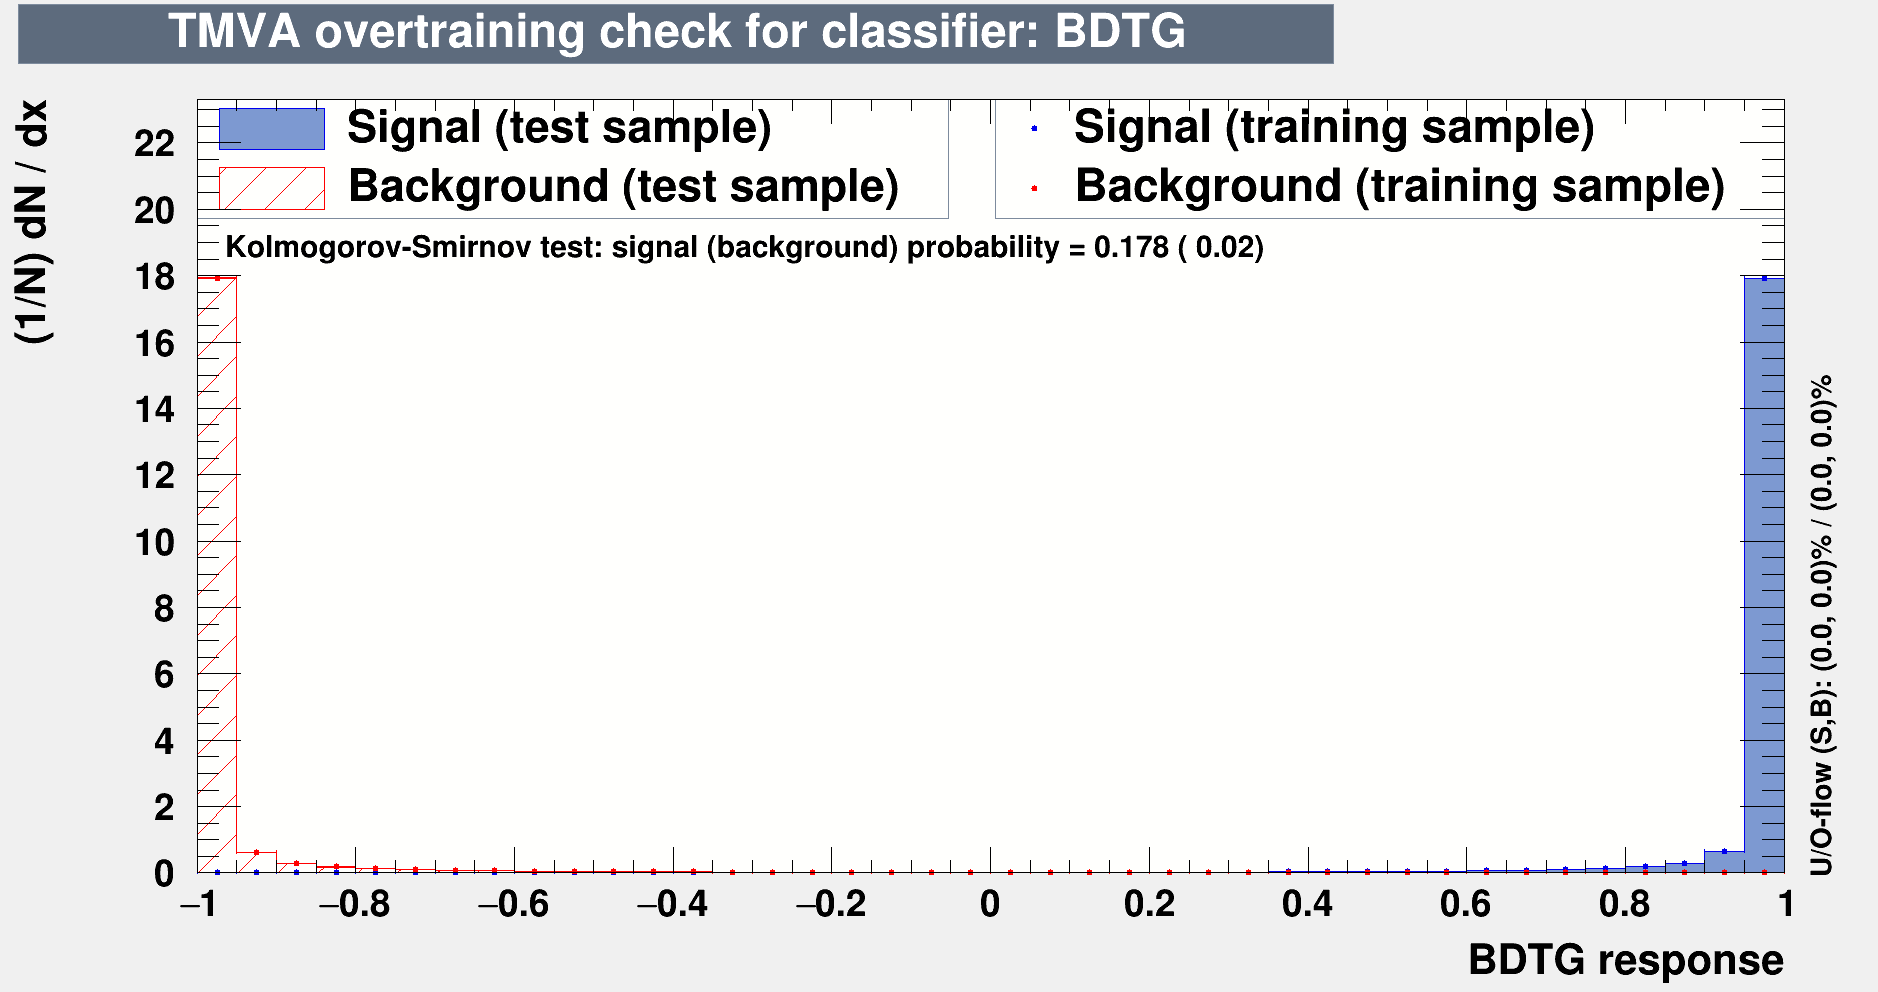
\includegraphics[width = 1.0\textwidth]{Plots/overtrain_BDTG.png}
      \caption{BDT output}
    \end{subfigure}%
    \begin{subfigure}{0.4\textwidth}
      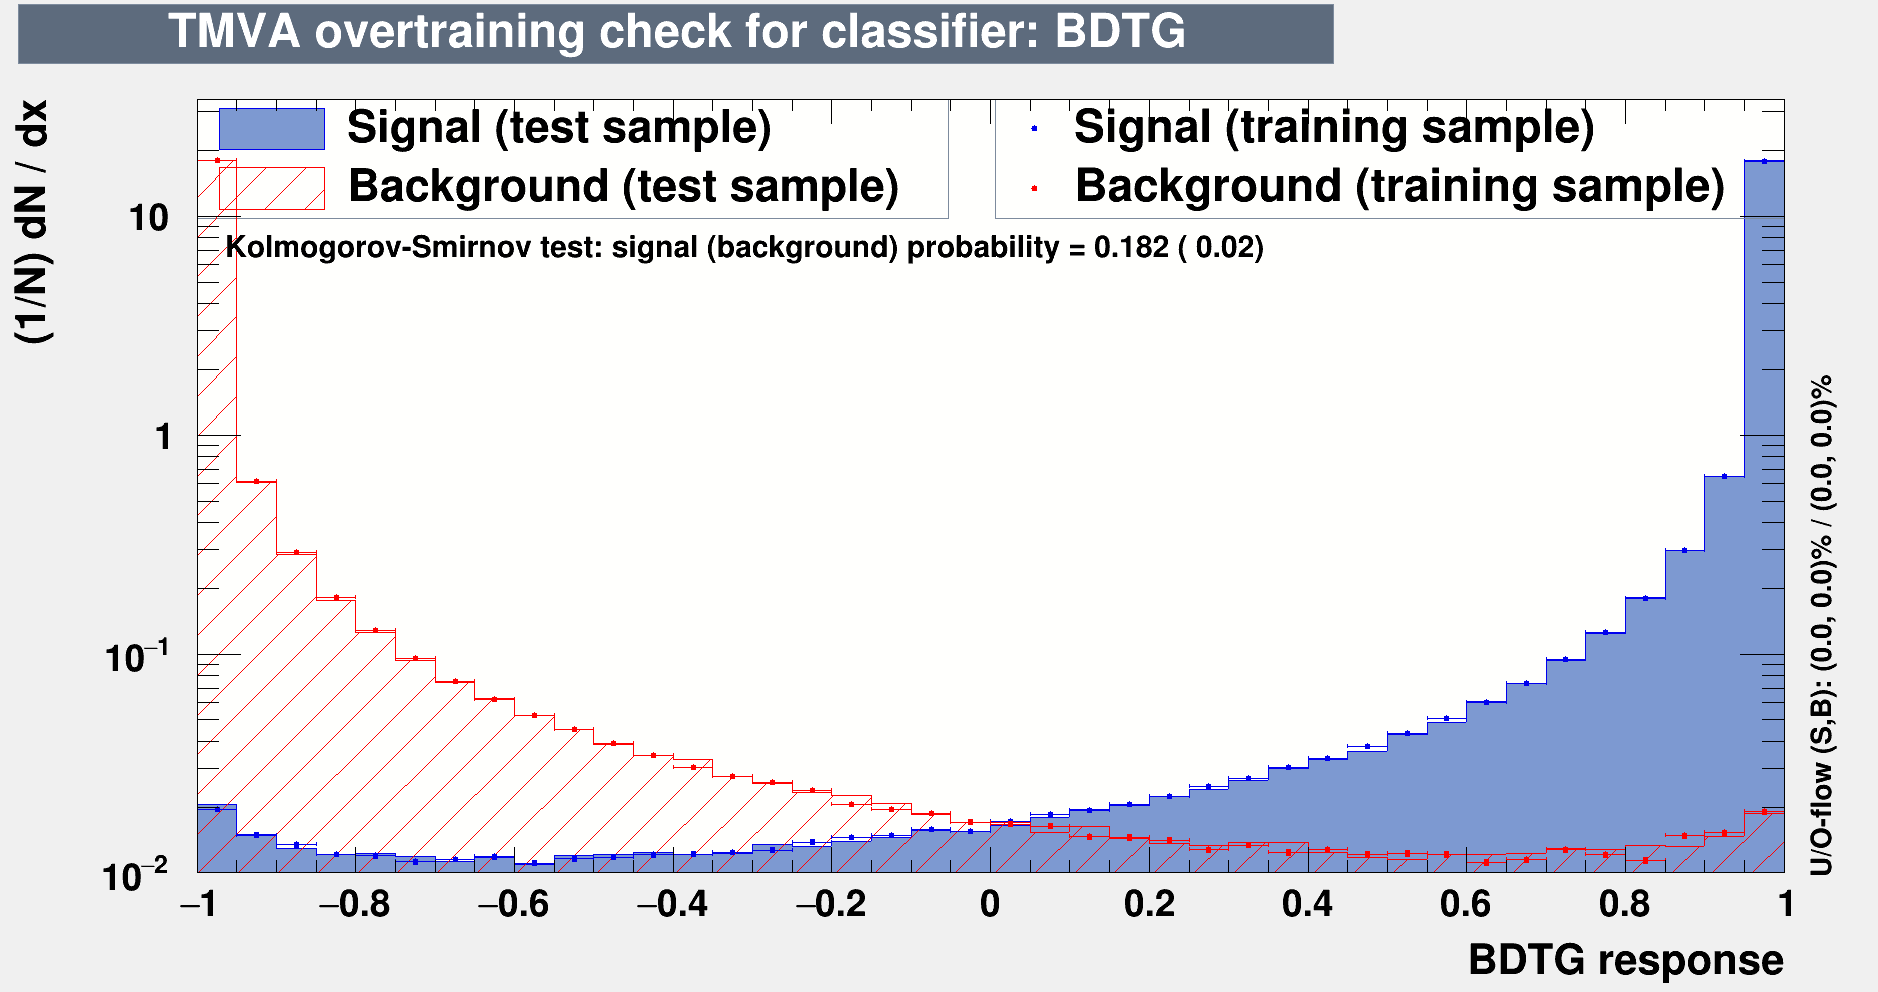
\includegraphics[width = 1.0\textwidth]{Plots/overtrain_BDTG_log.png}
      \caption{BDT output on a log scale}
    \end{subfigure}
  \end{figure}
\end{frame}

\section{Backgrounds}

\begin{frame}{Summary of backgrounds}
  \begin{itemize}
    \setlength\itemsep{1.0em}
    \item{Partially reconstructed $B$ decays}
    \begin{itemize}
      \item{Modelled in the fit with HILL/HORNSdini shapes}
    \end{itemize}
    \item{Combinatorial}
    \begin{itemize}
      \item{Floating exponential}
    \end{itemize}
    \item{CF $D^0\to K^-\pi^+\pi^-\pi^+$ and semi-leptonic $D^0\to K^-(X)l^+\nu_l$ background}
    \begin{itemize}
      \item{Small, assign systematic}
    \end{itemize}
    \item{Charmless}
    \begin{itemize}
      \item{Fix from sideband}
    \end{itemize}
    \item{CF $D^0\to K^-\pi^+\pi^-\pi^+\pi^0$ background}
    \begin{itemize}
      \item{Not negligible!}
    \end{itemize}
  \end{itemize}
\end{frame}

\begin{frame}{$D^0\to K^-\pi^+\pi^-\pi^+\pi^0$ partially reconstructed mis-ID}
  \begin{itemize}
    \setlength\itemsep{0.0em}
    \item{Missing $\pi^0$ and $\pi\to K$ mis-ID}
    \item{Float yield relative to $B\to D^*h$ background}
  \end{itemize}
  \begin{figure}
    \centering
    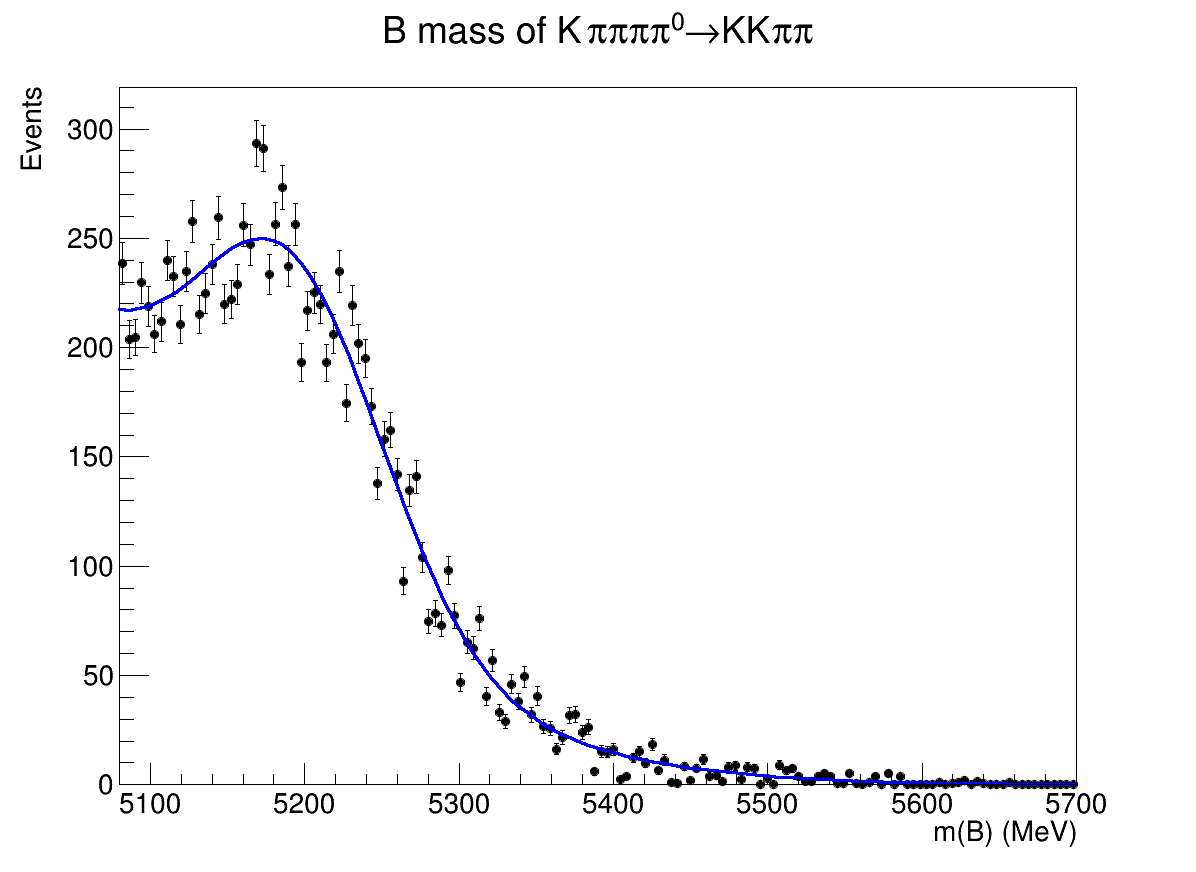
\includegraphics[width = 0.8\textwidth]{Plots/Kpipipipi0BMassB2DpiD2Kpipipi.png}
  \end{figure}
\end{frame}

\section{Global fit}

\begin{frame}{Global fit}
  \begin{figure}
    \centering
    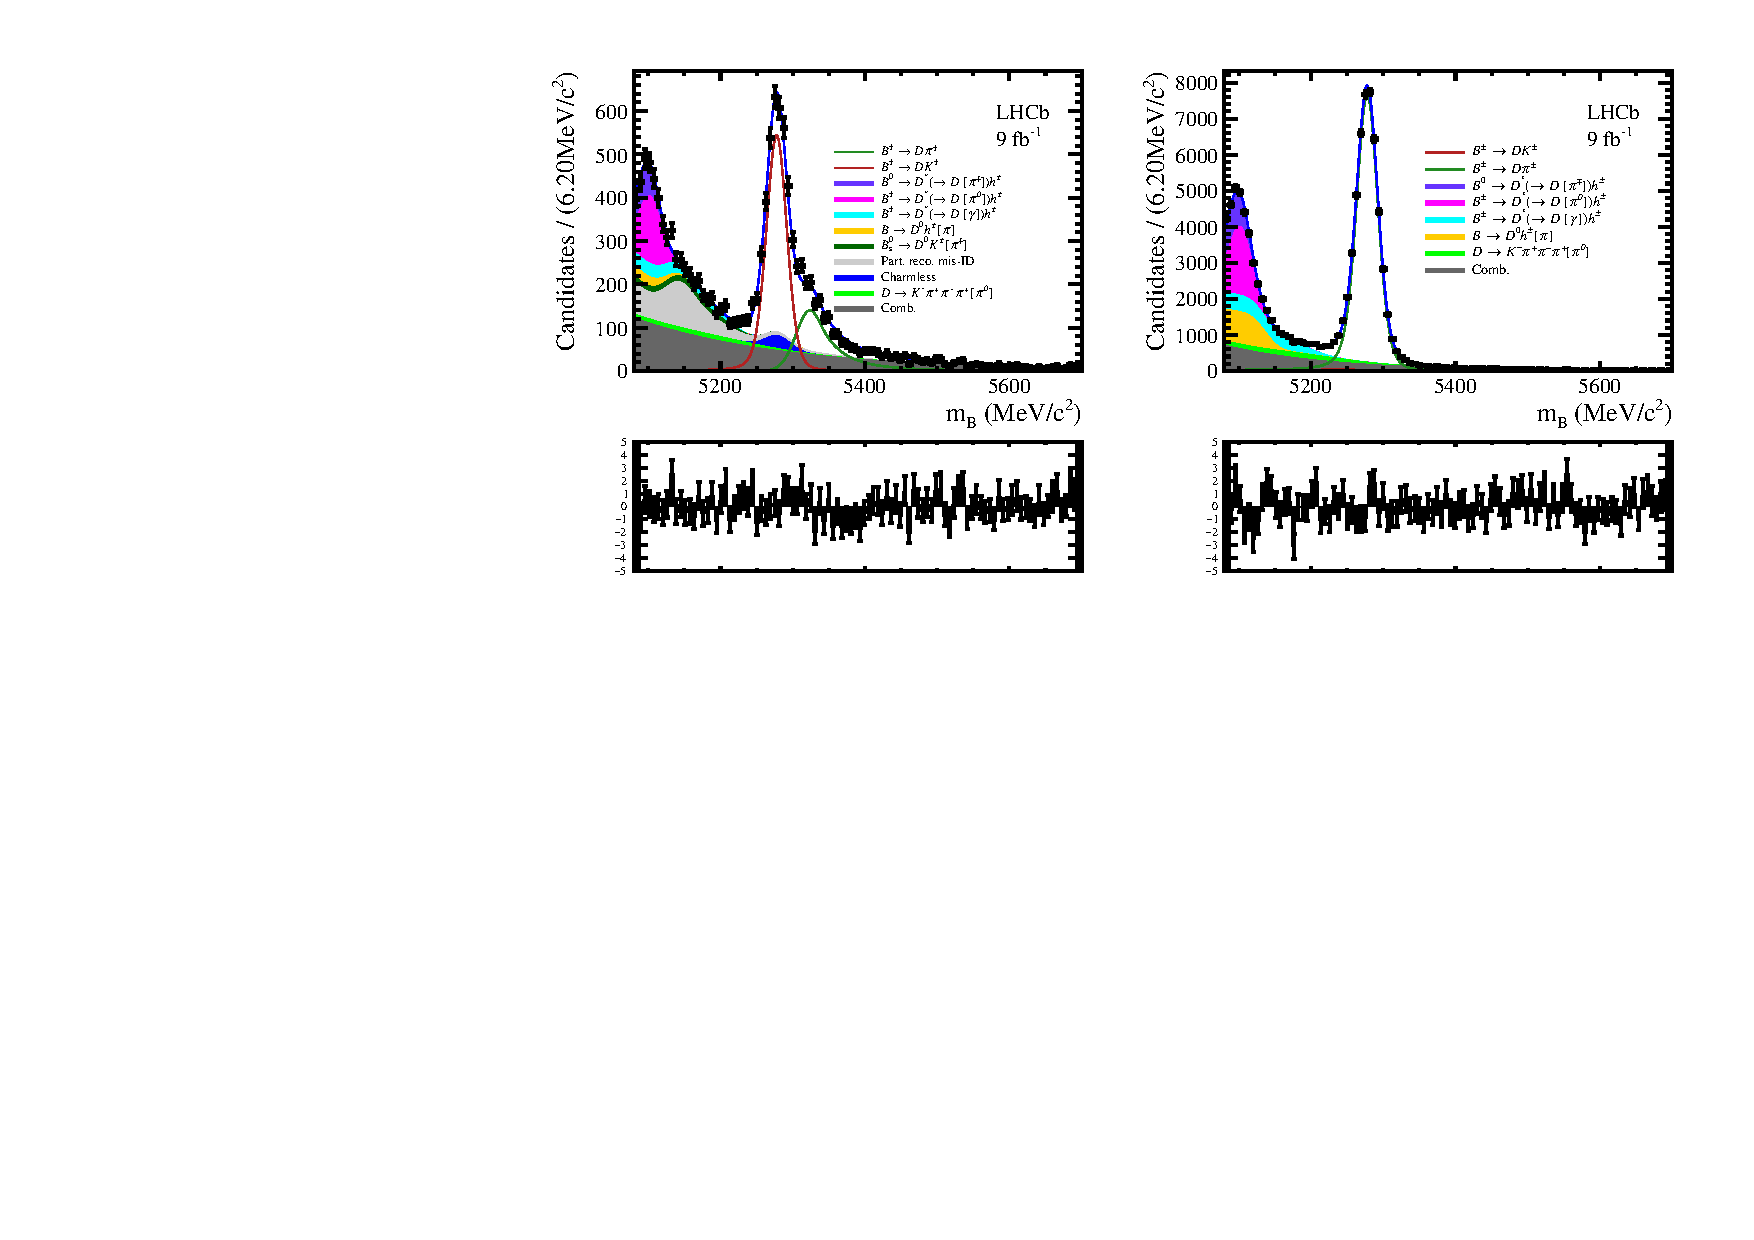
\includegraphics[width = 1.0\textwidth]{Plots/d2kkpipi_fiveL_allDP.pdf}
    \caption{$B^\pm\to DK^\pm$ channel (left) and $B^\pm\to D\pi^\pm$ channel (right)}
  \end{figure}
  \vspace{-0.5cm}
  \begin{itemize}
    \item{$B^\pm\to DK^\pm$ yield: $\SI{3026(38)}{}$}
    \item{$B^\pm\to D\pi^\pm$ yield: $\SI{44349(218)}{}$}
  \end{itemize}
\end{frame}

\section{Quasi-GLW fit}

\begin{frame}{Fit split by charge}
  \begin{figure}
    \centering
    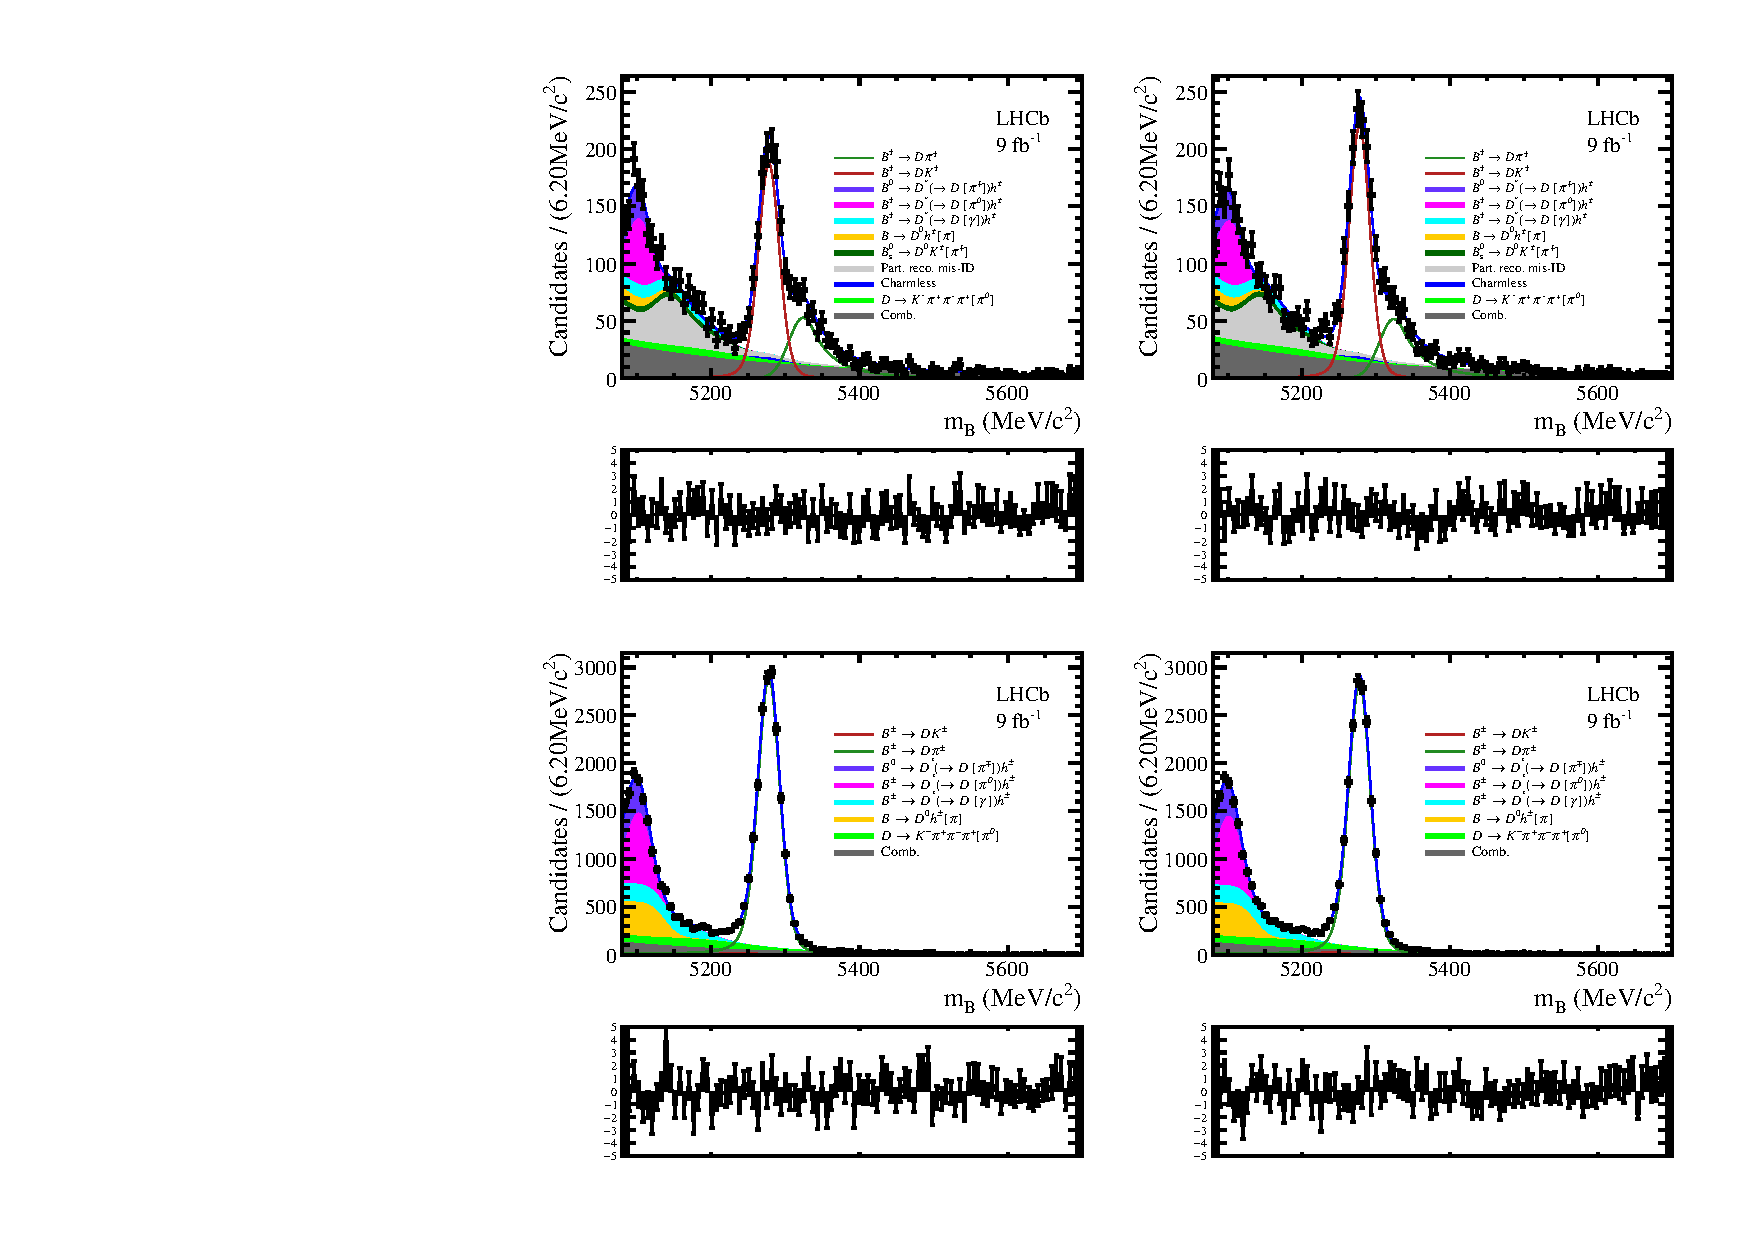
\includegraphics[width = 0.9\textwidth, clip = true, trim = {0 12.9cm 0 0}]{Plots/d2kkpipi_fiveL_allDP_GLW.pdf}
    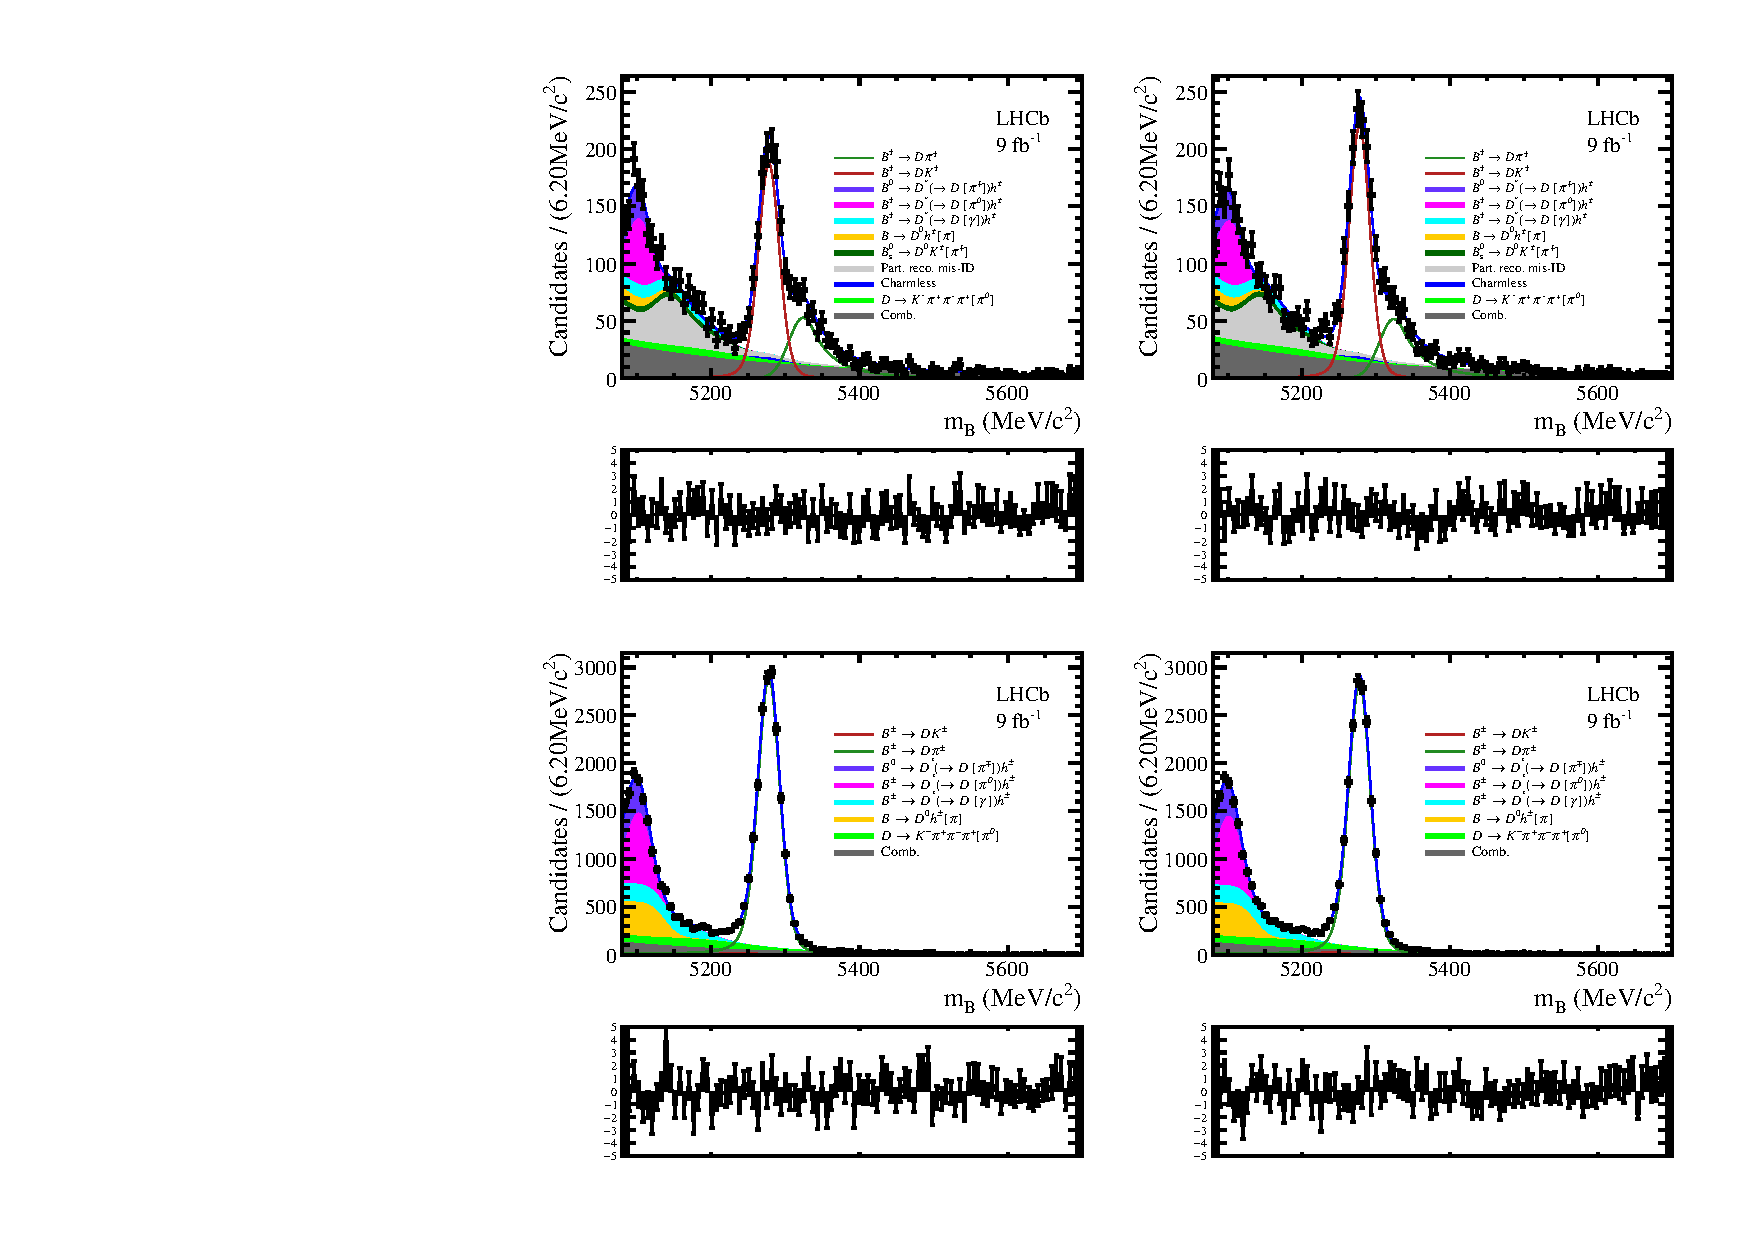
\includegraphics[width = 0.9\textwidth, clip = true, trim = {0 3cm 0 10cm}]{Plots/d2kkpipi_fiveL_allDP_GLW.pdf}
    \caption{$B^\pm\to (K^+K^-\pi^+\pi^-)Dh^\pm$}
  \end{figure}
\end{frame}

\begin{frame}{Fit split by charge}
  \begin{figure}
    \centering
    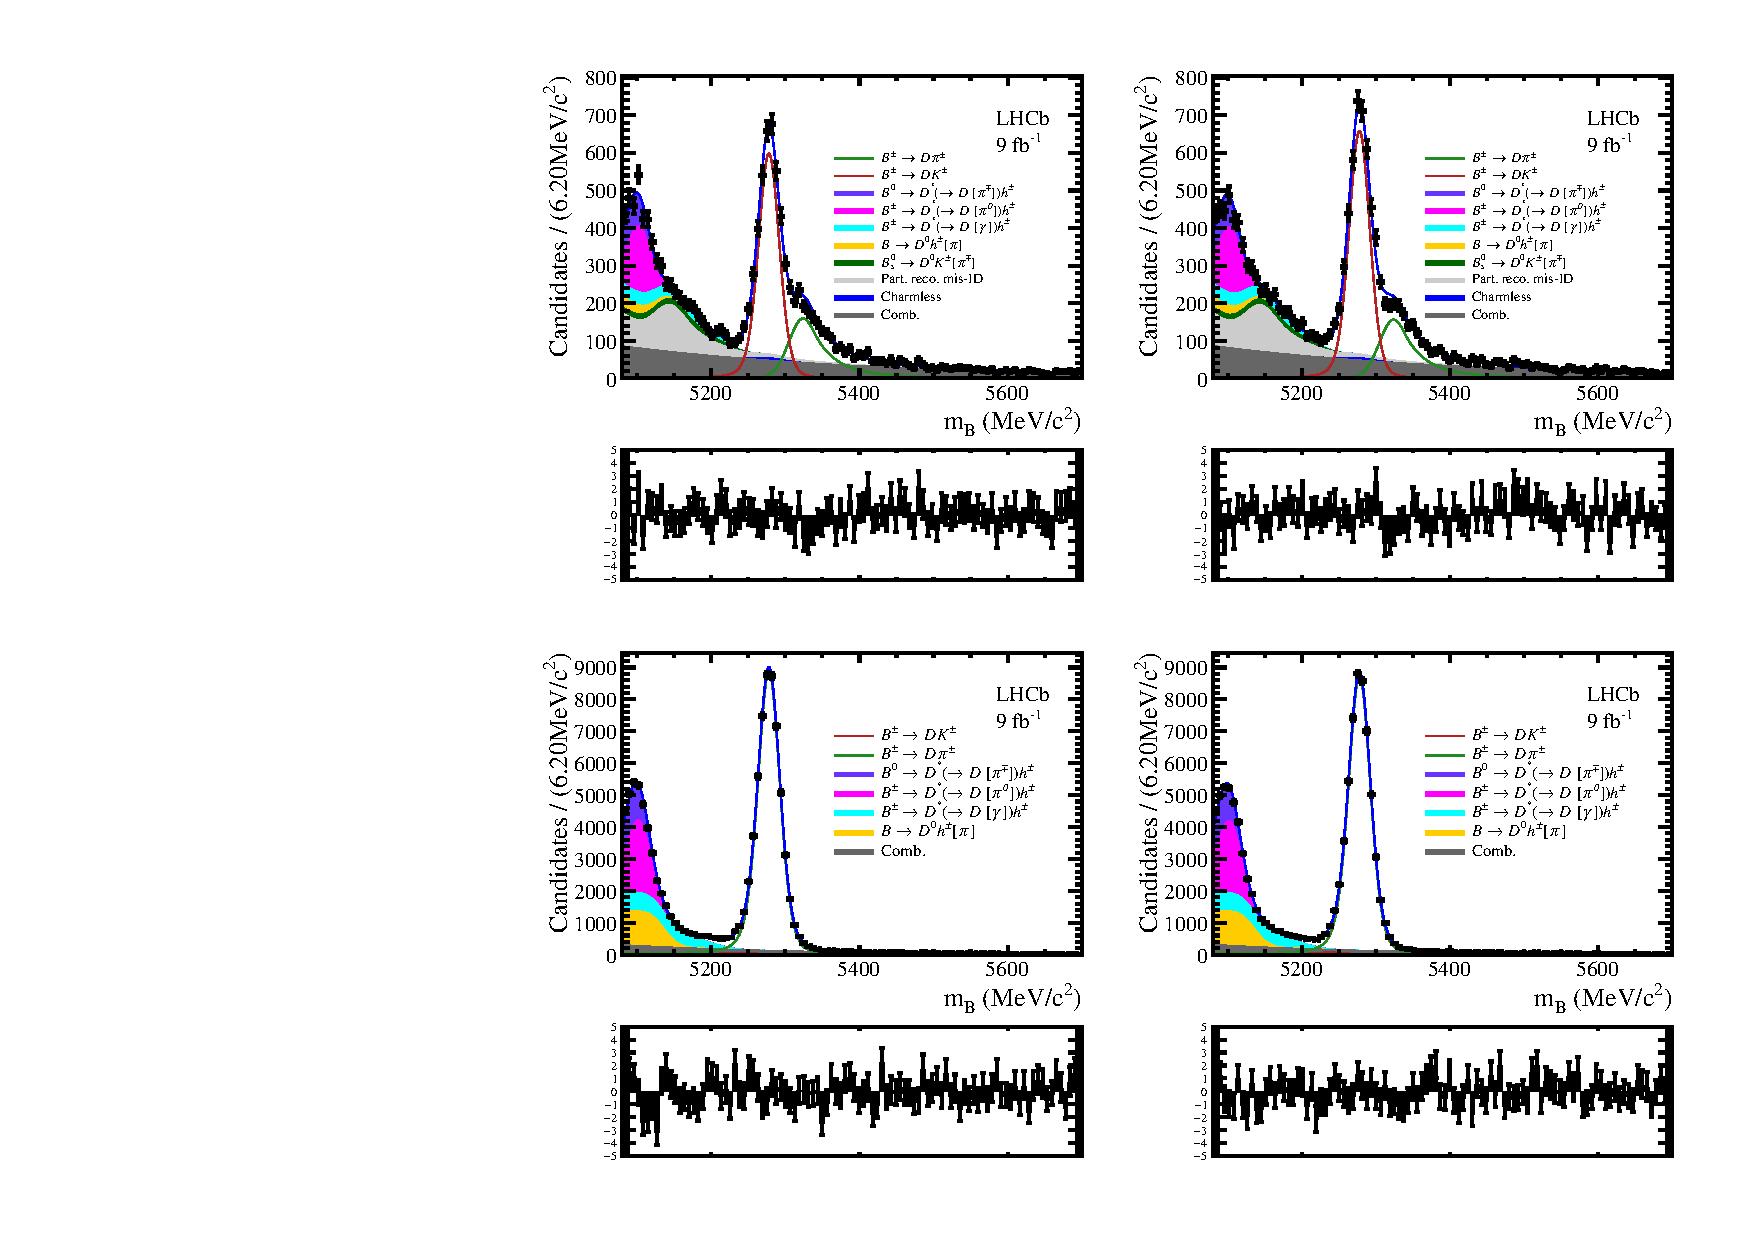
\includegraphics[width = 0.9\textwidth, clip = true, trim = {0 12.9cm 0 0}]{Plots/d2pipipipi_fiveL_allDP_GLW.pdf}
    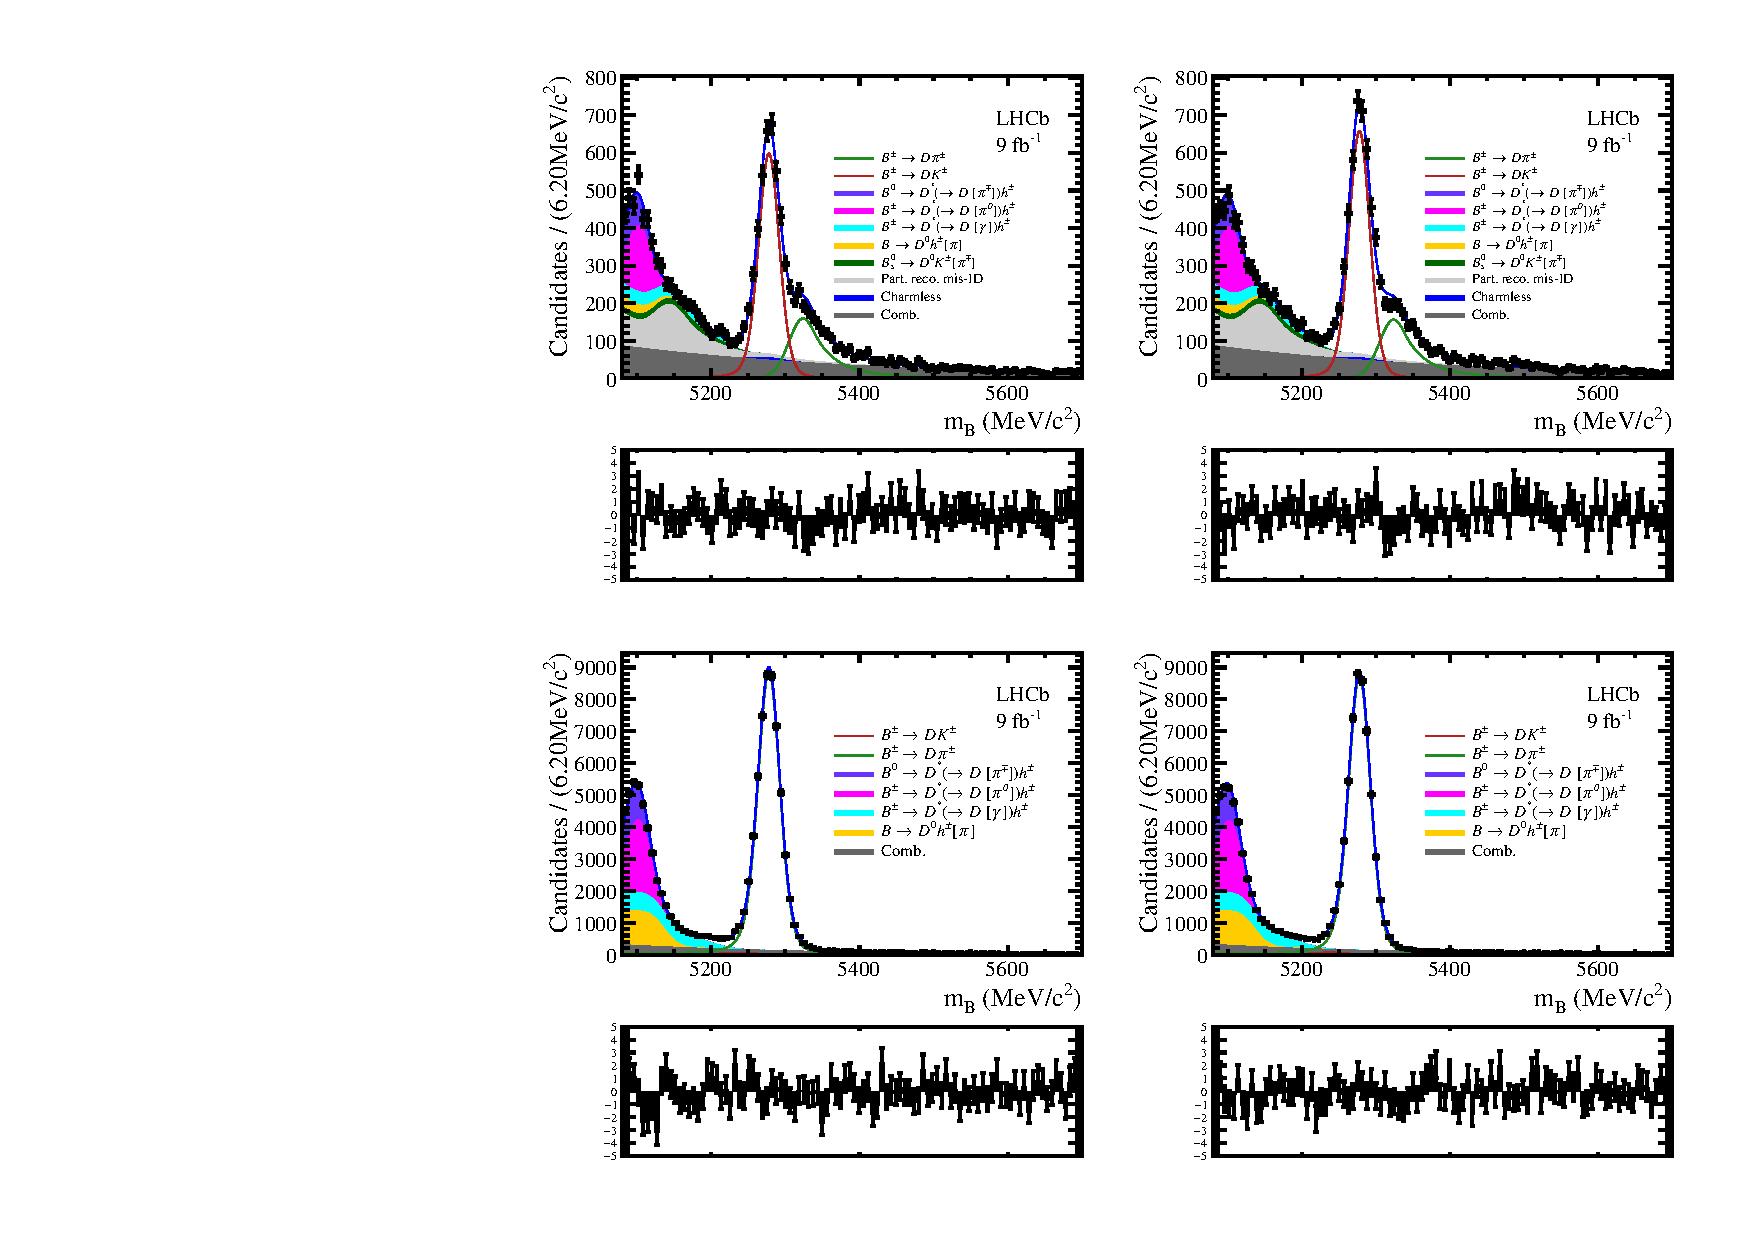
\includegraphics[width = 0.9\textwidth, clip = true, trim = {0 3cm 0 10cm}]{Plots/d2pipipipi_fiveL_allDP_GLW.pdf}
    \caption{$B^\pm\to (\pi^+\pi^-\pi^+\pi^-)Dh^\pm$}
  \end{figure}
\end{frame}

\section{CP fit}

\begin{frame}{CP fit setup}
  \begin{itemize}
    \setlength\itemsep{0.5em}
    \item{Fix mass shape from global fit}
    \item{Split by $B^\pm$ charge and $D$ phase space bins}
    \begin{itemize}
      \item{Simultaneous fit with $64$ categories}
    \end{itemize}
    \item{Signal yields parameterised in terms of CP observables $x_\pm^{DK}$, $y_\pm^{DK}$ $x_\xi^{D\pi}$, $y_\xi^{D\pi}$ ($6$ parameters)}
    \item{Fractional bin yields $F_i$ are floating ($15$ parameters)}
    \item{Combinatorial background yield floated in each bin ($64$ parameters)}
    \item{Total partially reconstructed background yield is floated in each bin ($64$ parameters)}
    \item{Normalisation of each charge and $B^\pm$ decay is floated ($4$ parameters)}
    \item{In total: $153$ free parameters}
  \end{itemize}
\end{frame}

\begin{frame}{CP fit results}
  \begin{figure}
    \centering
    \vspace{-0.2cm}
    \begin{subfigure}{0.5\textwidth}
      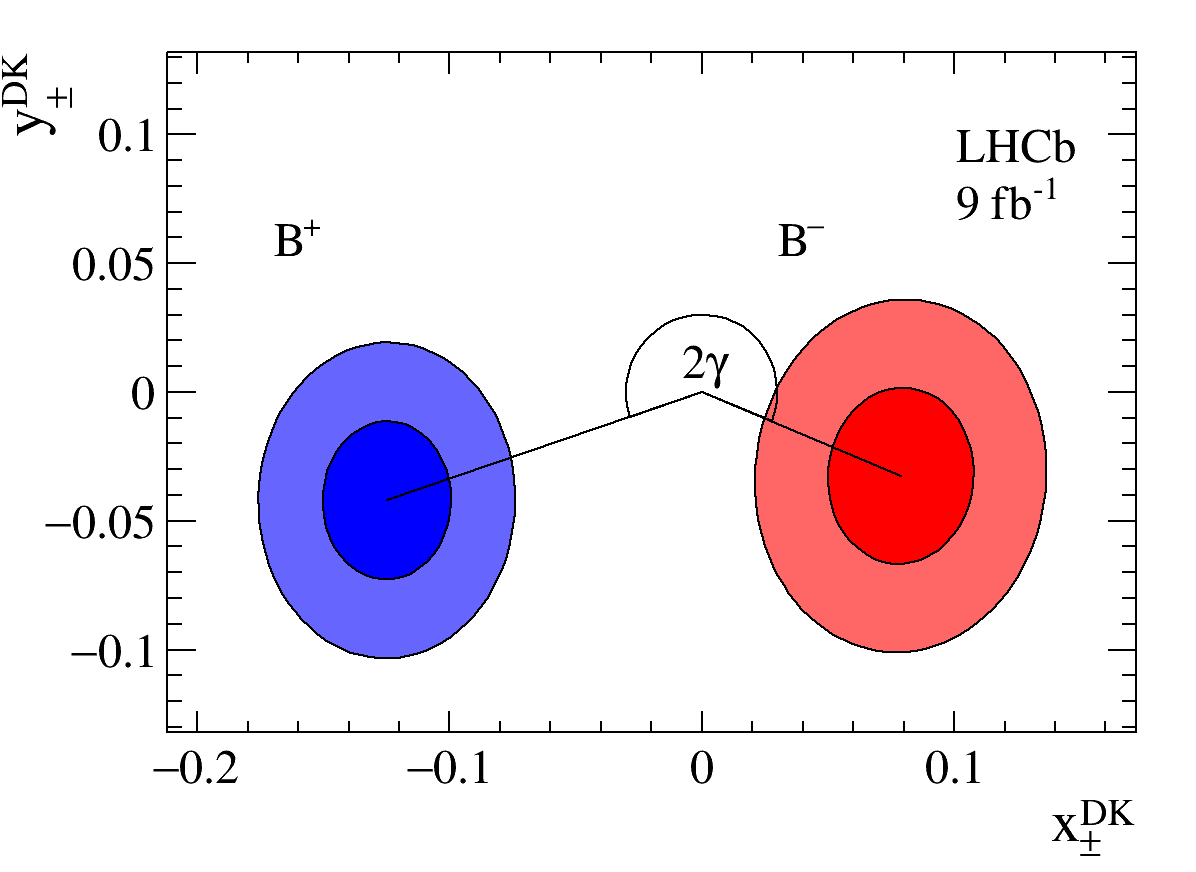
\includegraphics[width = 1.0\textwidth]{Plots/B2DK_CP_Observables_Contours.png}
      \caption{$x_\pm^{DK}$ vs $y_\pm^{DK}$}
    \end{subfigure}%
    \begin{subfigure}{0.5\textwidth}
      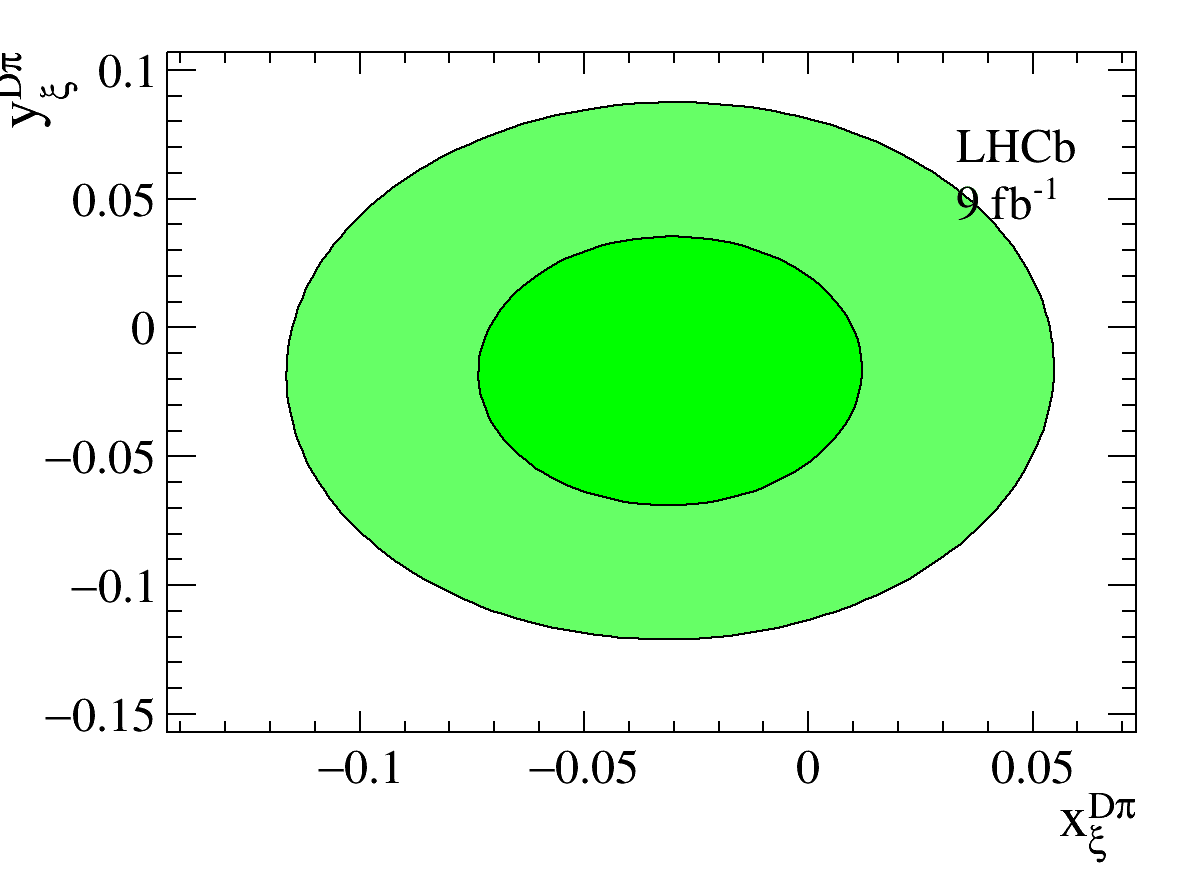
\includegraphics[width = 1.0\textwidth]{Plots/B2Dpi_CP_Observables_Contours.png}
      \caption{$x_\xi^{D\pi}$ vs $y_\xi^{D\pi}$}
    \end{subfigure}
  \end{figure}
  \vspace{-0.3cm}
  \begin{align*}
    x_\pm^{DK} = r_B\cos(\delta_B\pm\gamma) \\
    y_\pm^{DK} = r_B\sin(\delta_B\pm\gamma)
  \end{align*}
  \vspace{-0.5cm}
  \begin{itemize}
    \item{Shown are the $2\sigma$ contours of fitted CP observables}
    \item{The distinct $B^\pm\to DK^\pm$ contours indicate CP violation, while the $B^\pm\to D\pi^\pm$ mode has very low sensitivity to CP violation}
  \end{itemize}
\end{frame}

\begin{frame}{Fractional bin asymmetries}
  \begin{figure}
    \centering
    \vspace{-0.2cm}
    \begin{subfigure}{0.5\textwidth}
      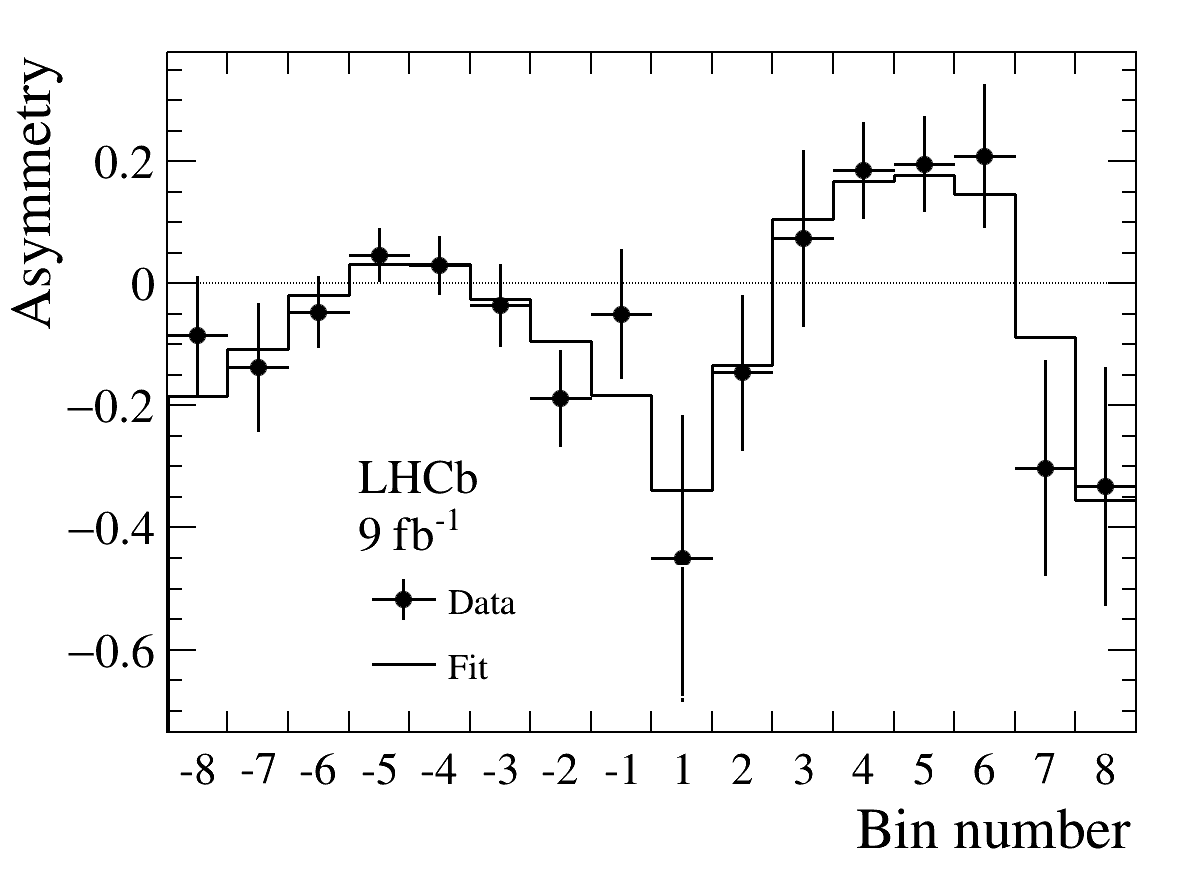
\includegraphics[width = 1.0\textwidth]{Plots/BinAsymmetries_dk.png}
      \caption{$B^\pm\to DK^\pm$}
    \end{subfigure}%
    \begin{subfigure}{0.5\textwidth}
      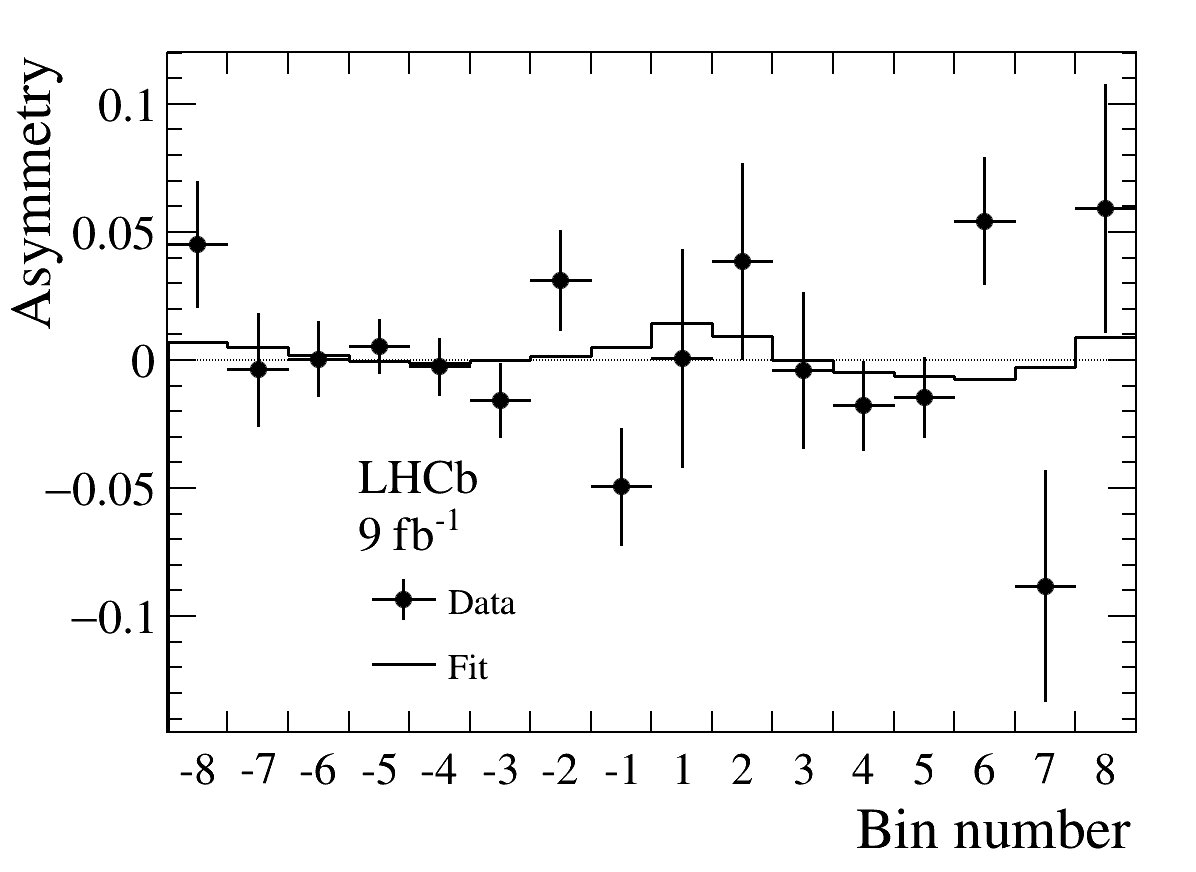
\includegraphics[width = 1.0\textwidth]{Plots/BinAsymmetries_dpi.png}
      \caption{$B^\pm\to D\pi^\pm$}
    \end{subfigure}
  \end{figure}
  \begin{itemize}
    \item{Useful cross check to compare measured bin asymmetries against bin asymmetries predicted by the fitted CP observables}
    \item{The $B^\pm\to DK^\pm$ mode show non-zero bin asymmetries, and the non-trivial distribution is driven by the change in strong phases across phase space}
  \end{itemize}
\end{frame}

\subsection{Systematic uncertainties}
\begin{frame}{Systematic uncertainties}
  \begin{itemize}
    \setlength\itemsep{1.0em}
    \item{Dominant $c_i$/$s_i$ systematic uncertainty due to model dependence}
    \begin{itemize}
      \item{Strategy: Generate toys with $c_i$/$s_i$ from older CLEO model, fit with $c_i$/$s_i$ from LHCb model}
      \item{Will be replaced when BESIII results become available}
    \end{itemize}
    \item{All internal systematic uncertainties are much smaller than the statistical uncertainties}
  \end{itemize}
\end{frame}

\begin{frame}{Summary of all BPGGSZ systematic uncertainties}
  \begin{center}
    Uncertainties of BPGGSZ CP observables in units of $10^{-2}$
  \end{center}
  \scriptsize
  \vspace{0.02cm}
  \begin{center}
    \begin{tabular}{lcccccc} 
        \hline
        Source & $x_-^{DK}$ & $y_-^{DK}$ & $x_+^{DK}$ & $y_+^{DK}$ & $x_\xi^{D\pi}$ & $y_\xi^{D\pi}$ \\
        \hline
        Statistical                                                & $2.87$ & $3.40$ & $2.51$ & $3.05$ & $4.24$ & $5.17$ \\
        \hline
        Mass shape                                                 & $0.02$ & $0.02$ & $0.03$ & $0.06$ & $0.02$ & $0.04$ \\
        Bin-dependent mass shape                                   & $0.11$ & $0.05$ & $0.10$ & $0.19$ & $0.68$ & $0.16$ \\ 
        PID efficiency                                             & $0.02$ & $0.02$ & $0.03$ & $0.06$ & $0.02$ & $0.04$ \\
        Low-mass background model                                  & $0.02$ & $0.02$ & $0.03$ & $0.04$ & $0.02$ & $0.02$ \\
        Charmless background                                       & $0.14$ & $0.15$ & $0.12$ & $0.14$ & $0.01$ & $0.02$ \\
        $C\!P$ violation in low-mass background                    & $0.01$ & $0.10$ & $0.08$ & $0.12$ & $0.07$ & $0.26$ \\
        Semi-leptonic $b$-hadron decays                            & $0.05$ & $0.27$ & $0.06$ & $0.01$ & $0.07$ & $0.19$ \\
        Semi-leptonic charm decays                                 & $0.02$ & $0.07$ & $0.03$ & $0.15$ & $0.06$ & $0.24$ \\
        $D\to K^-\pi^+\pi^-\pi^+$ background                       & $0.11$ & $0.05$ & $0.07$ & $0.04$ & $0.09$ & $0.05$ \\
        $\Lambda_b\to pD\pi^-$ background                          & $0.01$ & $0.25$ & $0.14$ & $0.04$ & $0.06$ & $0.34$ \\
        $D\to K^-\pi^+\pi^-\pi^+\pi^0$ background                  & $0.30$ & $0.05$ & $0.19$ & $0.07$ & $0.05$ & $0.01$ \\
        Fit bias                                                   & $0.06$ & $0.05$ & $0.13$ & $0.02$ & $0.06$ & $0.13$ \\
        \hline
        Total LHCb systematic                                      & $0.37$ & $0.43$ & $0.34$ & $0.32$ & $0.70$ & $0.57$ \\
        \hline
        $c_i$, $s_i$                                               & $0.35$ & $3.64$ & $1.74$ & $1.29$ & $0.14$ & $1.10$ \\
        \hline
        Total systematic                                           & $0.51$ & $3.67$ & $1.78$ & $1.33$ & $0.72$ & $1.24$ \\
        \hline
    \end{tabular}
  \end{center}
\end{frame}

\begin{frame}{Summary of all quasi-GLW systematic uncertainties}
  \begin{center}
    Uncertainties of quasi-GLW CP observables in units of $10^{-2}$
  \end{center}
  \footnotesize
  \vspace{0.02cm}
  \begin{center}
    \begin{tabular}{lcccccc} 
        \hline
        Source & $A_K^{KK\pi\pi}$ & $A_\pi^{KK\pi\pi}$ & $A_K^{\pi\pi\pi\pi}$ & $A_\pi^{\pi\pi\pi\pi}$ & $R_{C\!P}^{KK\pi\pi}$ & $R_{C\!P}^{\pi\pi\pi\pi}$ \\
        \hline
        Statistical                                   & $23.5$ & $5.5$ & $13.3$ & $3.1$ & $24.2$ & $14.3$ \\
        \hline
        Charmless background                          & $1.2$ & $<0.1$\phantom{00}  & $0.4$ & $<0.1$\phantom{00} & $13.9$ & $8.5$ \\
        External parameters                           & $1.0$ & $0.7$ & $1.0$ & $0.7$ & $4.0$ & $4.0$ \\
        Fixed yield fractions                         & $0.1$ & $<0.1$\phantom{00}  & $0.1$ & $<0.1$\phantom{00}  & $1.3$ & $1.4$ \\
        Mass shape                                    & $0.3$ & $<0.1$\phantom{00}  & $0.2$ & $<0.1$\phantom{00}  & $3.1$ & $3.1$ \\
        PID efficiency                                & $0.1$ & $<0.1$\phantom{00}  & $0.1$ & $<0.1$\phantom{00}  & $2.5$ & $1.6$ \\
        \hline
        Total systematic                              & $1.6$ & $0.7$ & $1.1$ & $0.7$ & $15.1$ & $10.1$ \\
        \hline
    \end{tabular}
  \end{center}
\end{frame}

\begin{frame}{Summary of measured CP observables}
  \vspace{-0.2cm}
  \begin{itemize}
    \item{Measured binned CP observables:}
  \end{itemize}
  \vspace{-0.2cm}
  \begin{align*}
    x_-^{DK} =& (7.9 \pm 2.9 \pm 0.4 \pm 0.4)\times 10^{-2} \\
    y_-^{DK} =& (-3.3 \pm 3.4 \pm 0.4 \pm 3.6)\times 10^{-2} \\
    x_+^{DK} =& (-12.5 \pm 2.5 \pm 0.3 \pm 1.3)\times 10^{-2} \\
    y_+^{DK} =& (-4.2 \pm 3.1 \pm 0.3 \pm 1.3)\times 10^{-2} \\
    x_\xi^{D\pi} =& (-3.1 \pm 4.3 \pm 0.7 \pm 0.1)\times 10^{-2} \\
    y_\xi^{D\pi} =& (-1.7 \pm 5.2 \pm 0.6 \pm 1.1)\times 10^{-2}
  \end{align*}
  \vspace{-0.7cm}
  \begin{itemize}
    \item{Measured inclusive CP observables:}
  \end{itemize}
  \vspace{-0.2cm}
  \begin{align*}
    A_K^{KK\pi\pi} =& 0.093 \pm 0.023 \pm 0.002 \\
    A_\pi^{KK\pi\pi} =& -0.009 \pm 0.006 \pm 0.001 \\
    A_K^{\pi\pi\pi\pi} =& 0.060 \pm 0.013 \pm 0.001 \\
    A_\pi^{\pi\pi\pi\pi} =& -0.0082 \pm 0.0031 \pm 0.0007 \\
    R_{\rm CP}^{KK\pi\pi} =& 0.974 \pm 0.024 \pm 0.015 \\
    R_{\rm CP}^{\pi\pi\pi\pi} =& 0.978 \pm 0.014 \pm 0.010
  \end{align*}
\end{frame}

\section{Interpretation}

\begin{frame}{Interpretation}
  \begin{figure}
    \centering
    \begin{subfigure}{0.50\textwidth}
      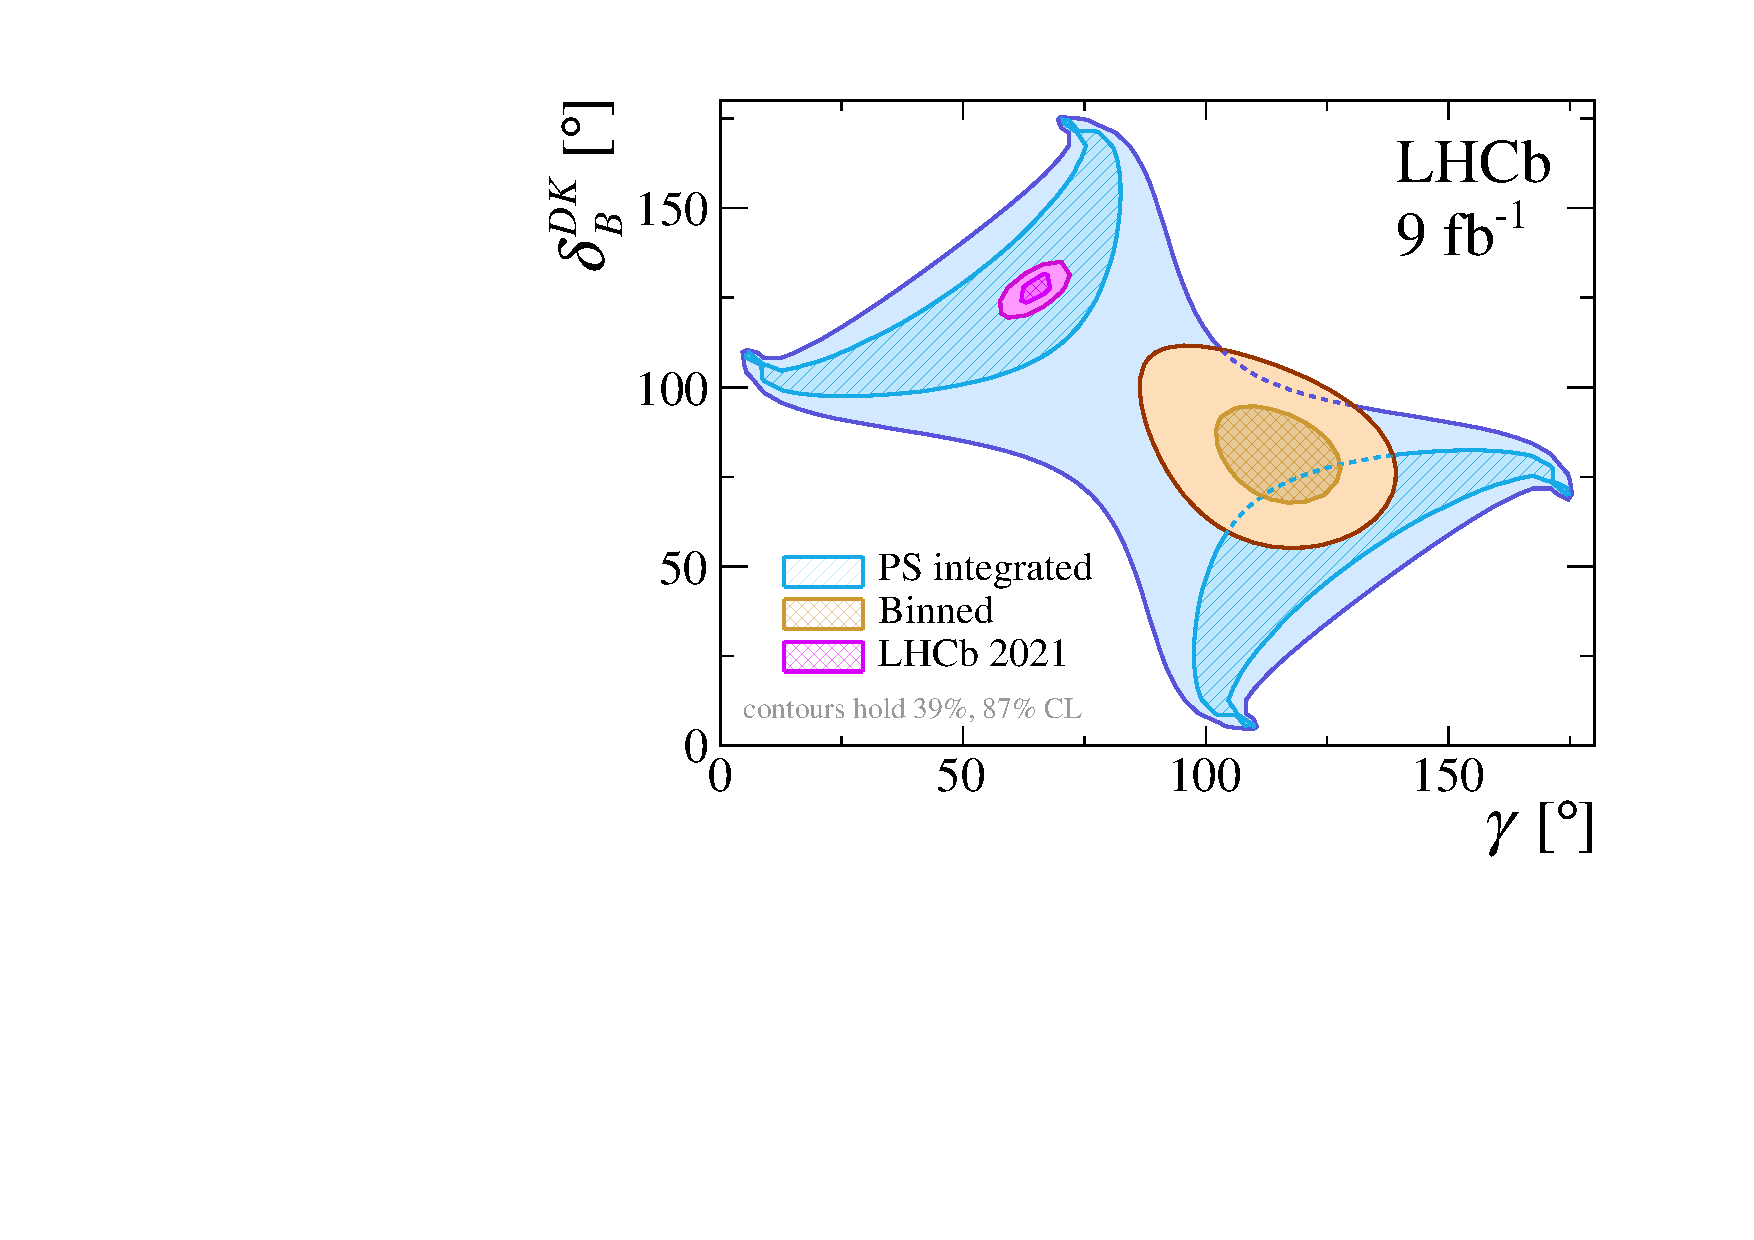
\includegraphics[width = 1.0\textwidth]{Plots/gammacharm_lhcb_KKpipi_GLW_KKpipi_GGSZ_lhcb_2020_beauty_and_charm_g_d_dk.pdf}
    \end{subfigure}%
    \begin{subfigure}{0.50\textwidth}
      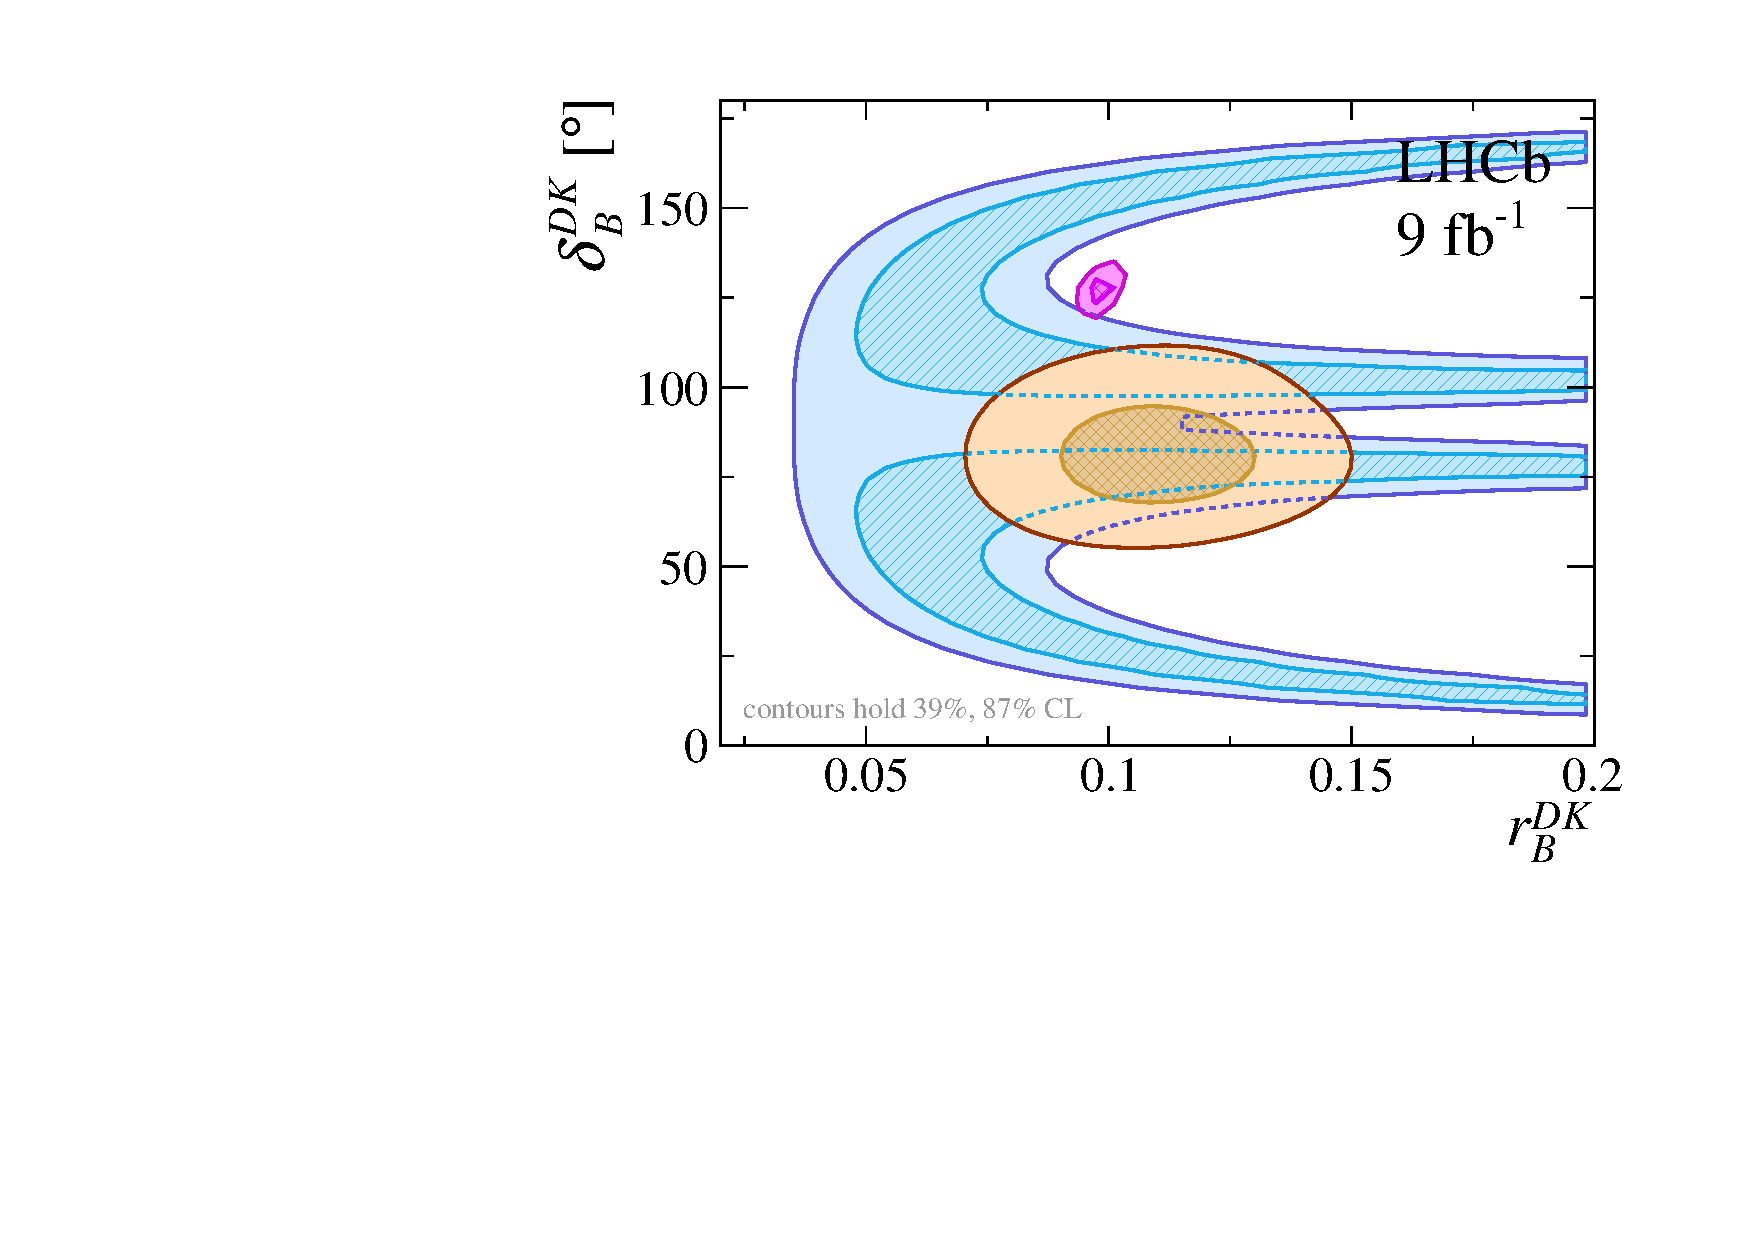
\includegraphics[width = 1.0\textwidth]{Plots/gammacharm_lhcb_KKpipi_GLW_KKpipi_GGSZ_lhcb_2020_beauty_and_charm_r_dk_d_dk.pdf}
    \end{subfigure}
  \end{figure}
  \vspace{-0.75cm}
  Results from binned fit:
  \begin{align*}
    \gamma &= (116^{+12}_{-14})^\circ \\
    \delta_B^{DK} &= (81^{+14}_{-13})^\circ \\
    r_B^{DK} &= 0.110^{+0.020}_{-0.020} \\
    \delta_B^{D\pi} &= (298^{+62}_{-118})^\circ \\
    r_B^{D\pi} &= 0.0041^{+0.0055}_{-0.0041}
  \end{align*}
\end{frame}

\begin{frame}{Interpretation}
  \begin{figure}
    \centering
    \begin{subfigure}{0.50\textwidth}
      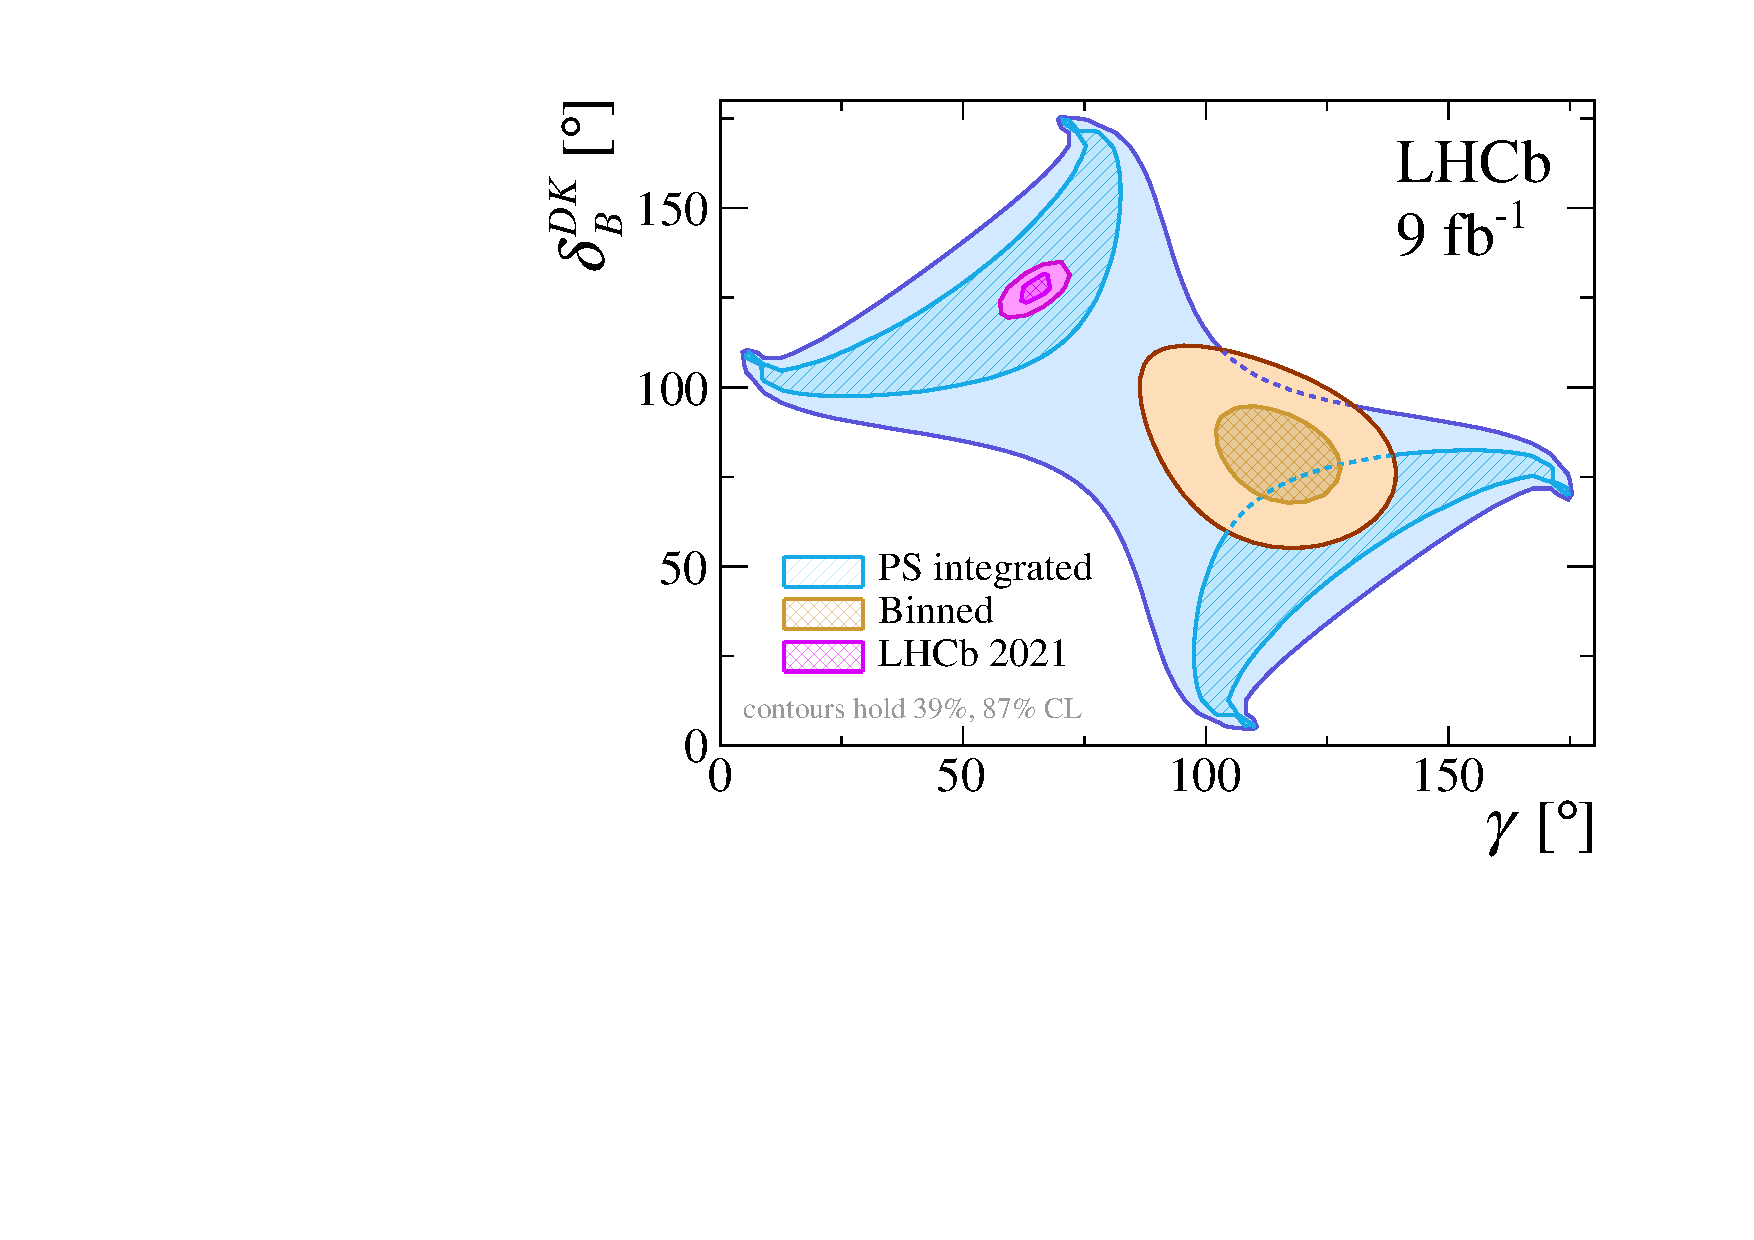
\includegraphics[width = 1.0\textwidth]{Plots/gammacharm_lhcb_KKpipi_GLW_KKpipi_GGSZ_lhcb_2020_beauty_and_charm_g_d_dk.pdf}
    \end{subfigure}%
    \begin{subfigure}{0.50\textwidth}
      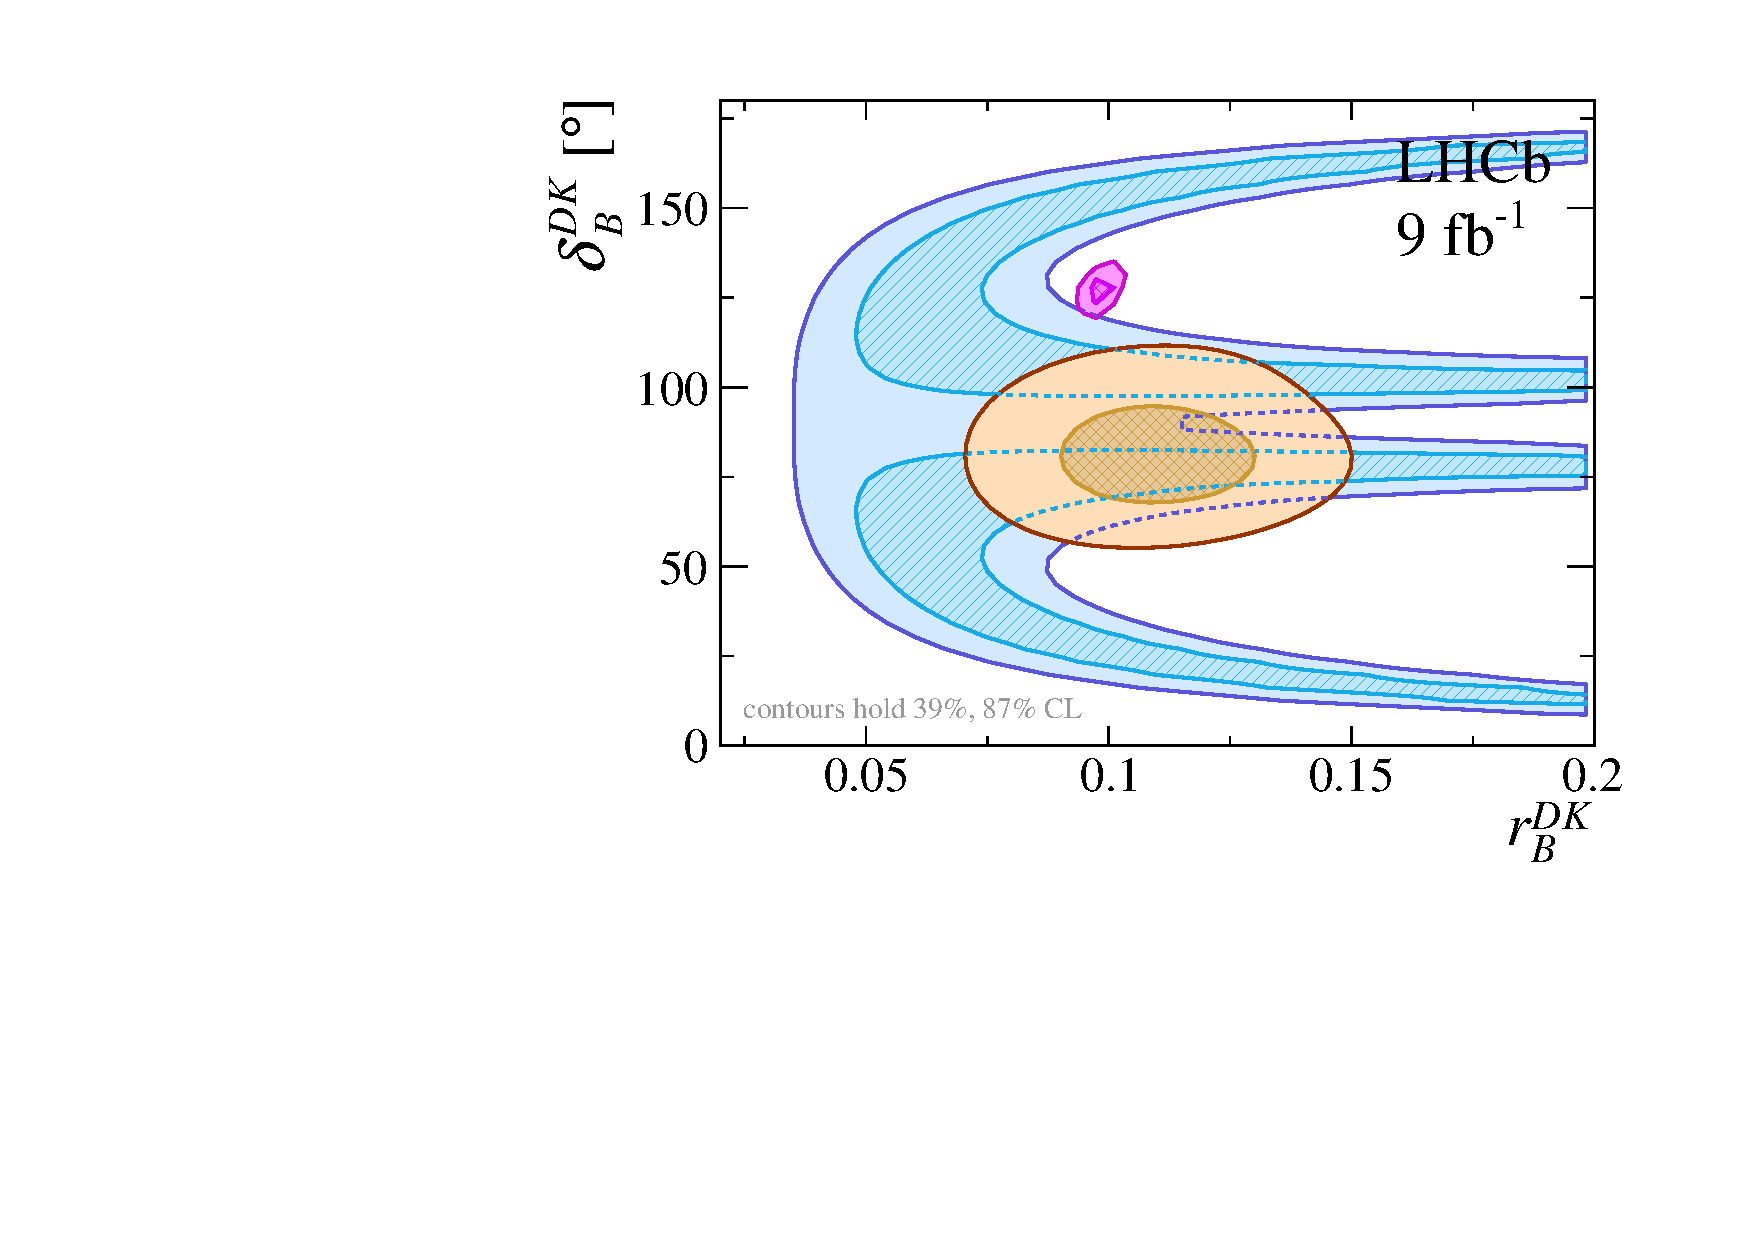
\includegraphics[width = 1.0\textwidth]{Plots/gammacharm_lhcb_KKpipi_GLW_KKpipi_GGSZ_lhcb_2020_beauty_and_charm_r_dk_d_dk.pdf}
    \end{subfigure}
  \end{figure}
  \vspace{-0.35cm}
  \begin{itemize}
    \item{Value of $\gamma$ from binned analysis is somewhat high, but falls within the $3\sigma$ contours}
    \item{Phase space inclusive measurement are compatible with our expectations}
    \item{Interpretation may evolve when full model independent inputs are available}
  \end{itemize}
\end{frame}

\section{Conclusion}

\begin{frame}{Conclusion}
  \begin{itemize}
    \setlength\itemsep{0.5em}
    \item{First study of CP violation has been performed in $B^\pm\to[K^+K^-\pi^+\pi^-]_D h^\pm$ in bins of phase space}
    \item{Phase space inclusive measurement for $B^\pm\to[K^+K^-\pi^+\pi^-]_D h^\pm$ and $B^\pm\to[\pi^+\pi^-\pi^+\pi^-]_D h^\pm$}
    \item{This publication is model dependent, but strong phases will become available from BESIII soon}
    \begin{itemize}
      \item{Sufficient information will be provided in the paper to allow a model independent update when $c_i$ and $s_i$ become available}
    \end{itemize}
    \item{Complete paper draft is available}
    \item{Link to:}
    \begin{itemize}
      \item{\href{https://twiki.cern.ch/twiki/bin/viewauth/LHCbPhysics/GGSZB2DhD2hhpipiModelIndependent}{TWiki}}
      \item{\href{https://twiki.cern.ch/twiki/pub/LHCbPhysics/GGSZB2DhD2hhpipiModelIndependent/LHCb-ANA-2021-051-v9.pdf}{ANA note}}
      \item{\href{https://twiki.cern.ch/twiki/pub/LHCbPhysics/GGSZB2DhD2hhpipiModelIndependent/LHCb-PAPER-2022-XXX-v0.pdf}{Paper draft} (also uploaded to Indico)}
    \end{itemize}
  \end{itemize}
  \begin{center}
    \huge Thanks for listening!
  \end{center}
\end{frame}

\end{document}